\section{Computational Results}\label{sec:compResults}
In this section we show several computational experiments using state
redistribution to solve the Euler
equations. We will also use these
examples to examine 
properties of different gradient choices and base schemes. 
%We solve the conservation law \eqref{eq:conslaw2D} with different fluxes $\mathbf{F}$, to include both smooth and discontinuous
%solutions.

%\subsection{Linear fluxes}
%\subsubsection{Linear convergence study}
%We solve \eqref{eq:conslaw2D} with the flux $\mathbf{F}(u) = [-2\pi y u, 2\pi x u]$ and initial condition
%$$
%u_0(x,y) = w(\theta - \pi/2)
%$$
%where
%$$
%w(\theta) = \frac{1}{2}\left( \text{erf}\left( \frac{\pi/6 - \theta}{\sqrt{4/100}} \right) + \text{erf}\left( \frac{\pi/6 + \theta}{\sqrt{4/100}} \right)\right)
%$$
%until the final time $T = 1$ on the domain enclosed by two concentric disks of 
%radii $R_1 = 0.751$ and $R_2 = 1.251$.  
%Figure \ref{fig:rotatinghillgrid} shows the computational domain 
%embedded in a $50 \times 50$ grid.  The exact solution is the initial condition 
%rotated about the point $(1.5,1.5)$, where $T=1$ corresponds to one solid 
%body rotation. This example IS FROM \cite{}, for comparison.  (AND ADD
%COMPARISON - ARE THEY OR WE MORE ACCURATE< BUT WE ARE EASIER).   
%The errors 
%measured in the $L_1$ and $L_\infty$ norms are provided in 
%Tables \ref{tab:ex1_L1} and \ref{tab:ex1_Linf}.  Figure
%\ref{fig:rotatinghillexactiso} shows isolines of solution at the initial 
%and final time.  The exact solution is applied as the boundary condition.
%CHEATING?
%This problem is solved using the finite volume TVD-RK2 scheme. 
%
%\begin{figure}
%\subfloat[$50\times50$ grid and annulus domain.]{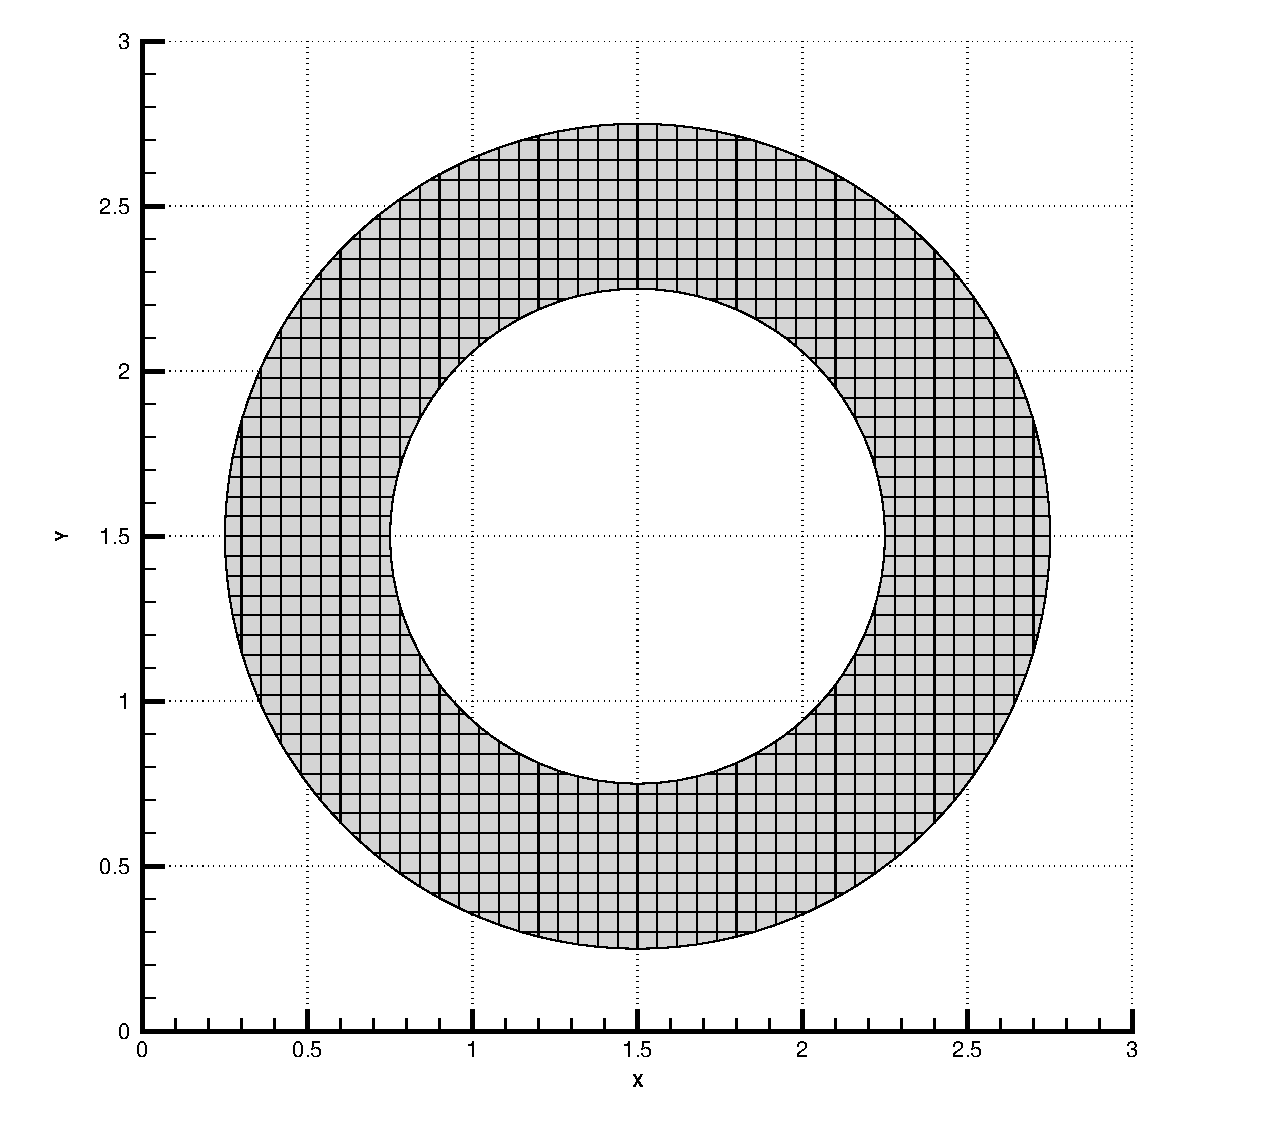
\includegraphics[width = 0.5\linewidth]{figs/rotatinghill_grid.eps} \label{fig:rotatinghillgrid}} 
%\quad
%\subfloat[Isolines of exact solution at the initial and final time. SHOW
%COMPUTED SOLUTION TOO]{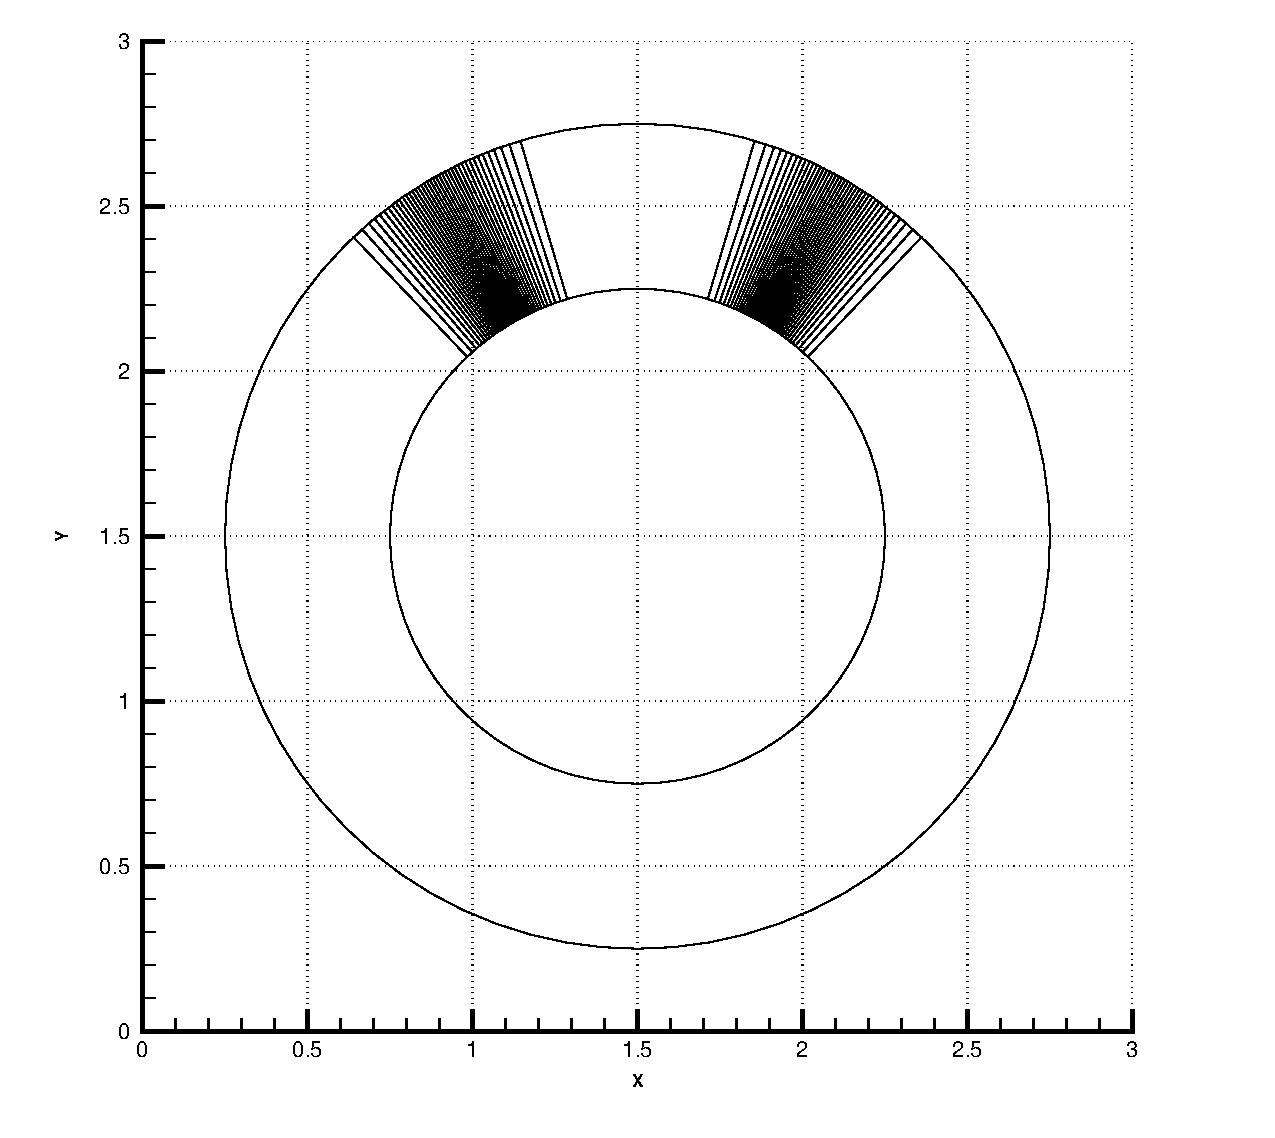
\includegraphics[width = 0.5\linewidth]{figs/rotatinghill_solution.eps}\label{fig:rotatinghillexactiso}}
%\end{figure}
%    % \caption{}\label{tab:ex1_L1}
%
%{\large
%\begin{table}
%\centering
%\subfloat[$L_1$ errors. \label{tab:ex1_L1}]{
%    \begin{tabular}{|c|c|c|c|c|}
%        \hline
%         $N_x \times N_y$ & $p = 0$ & $p=1$& $p=2$ & $p=3$ \\
%         \hline
%         50 & 2.3937e-1(-) &  5.6588e-2  (-)& 4.1690e-2  (-)&   2.0694e-2 (-)\\
%         \hline
%         100 &  1.5521e-1 (0.62) &  2.0125e-2  (1.49)& 7.8165e-3 (2.41)& 1.6813e-3 (3.62)\\
%         \hline
%         200 &  9.4138e-2 (0.72) & 5.5222e-3 (1.86)&  9.98411e-4 (2.96)& 8.8527e-5 (4.24)\\
%        %  \hline
%        %  400 &  () &  ()&  ()&  ()\\
%         \hline
%    \end{tabular}
%    }
%\quad
%\subfloat[$L_\infty$ errors. \label{tab:ex1_Linf}]{
%    \begin{tabular}{|c|c|c|c|c|}
%        \hline
%         $N_x \times N_y$ & $p = 0$ & $p=1$& $p=2$ & $p=3$ \\
%         \hline
%         50 & 3.0385e-1 (-) &  1.6856e-1 (-)& 1.1809e-1 (-)&  7.0682e-2 (-)\\
%         \hline
%         100 & 2.3332e-1 (0.38) & 8.5487e-2 (1.04)& 5.1249e-2 (1.20)& 1.6657e-2 (2.08)\\
%         \hline
%         200 &  1.7698e-1 (0.39) & 3.4940e-2 (1.29)& 1.4500e-2 (1.82)&  1.9507e-3 (3.09)\\
%        %  \hline
%        %  400 &   () &  ()&  ()&  ()\\
%         \hline
%    \end{tabular}
%    }
%
%\caption{Errors for the linear convergence study. ADD METHOD DETAILS TO
%DESCRIPTION - USED WHICH GRADIENT RECON. ADD 400 POINTS}
%\end{table}
%}
%
%\subsubsection{Overlapping neighborhoods}
%The purpose of this example is to demonstrate that our algorithm can handle a substantial number of overlapping neighborhoods.  
%Using the streamfunction
%$$
%\phi = R - 0.25\sin(10\theta),
%$$
%with $R = \sqrt{(x-1.5)^2+(y-1.5)^2}$ and $\theta = \arctan((y-1.5)/(x-1.5))$, we define a linear flux based on the resulting divergence free velocity field, i.e.,  $\mathbf{F}(u) = [\phi_y u, -\phi_xu]$.  The characteristics of \eqref{eq:conslaw} lie on the isolines of the streamfunction.
%
%A steady state solution to \eqref{eq:conslaw} with the above flux is given by the streamline function.  Therefore, we start with the initial condition given by the streamline function $\phi$, and compute the solution until the final time $T = 10$ on a $100 \times 100$ grid.  Additionally, we set the flux normal the domain boundary $\mathbf{F}\cdot \mathbf{n} = 0$.  This is to ensure that information does not leave the domain and should solution growth occur, this will more easily be noticed.
%This problem is solved using the finite volume TVD-RK2 scheme. 
%
%
%\begin{table}[h]
%    \centering
%    \subfloat[$L_1$ errors.]{
%    \begin{tabular}{|c|c|c|c|}
%    \hline
%        $p = 0$ & $p =1$ & $p = 2$ & $p =3$  \\
%        \hline
%        3.8585e-1 & 3.6118e-2 & 8.29907e-3 & 4.3116e-3\\
%        \hline
%    \end{tabular} \label{tab:errorsteadystatel1}
%    }
%    \quad
%\subfloat[$L_\infty$ errors.]{
%    \begin{tabular}{|c|c|c|c|}
%    \hline
%        $p = 0$ & $p =1$ & $p = 2$ & $p =3$  \\
%        \hline
%        2.9470e-1 & 9.5323e-2 & 2.4851e-2 &  5.4720e-3 \\
%        \hline
%    \end{tabular}
%    \label{tab:errorsteadystatelinfty}
%    }
%    
%\caption{Errors for overlapping neighborhoods study.} \label{tab:overlappingerrors}
%\end{table}
%
%\begin{figure}[h]
%%\subfloat[Isolines of exact solution at the initial and final time.]{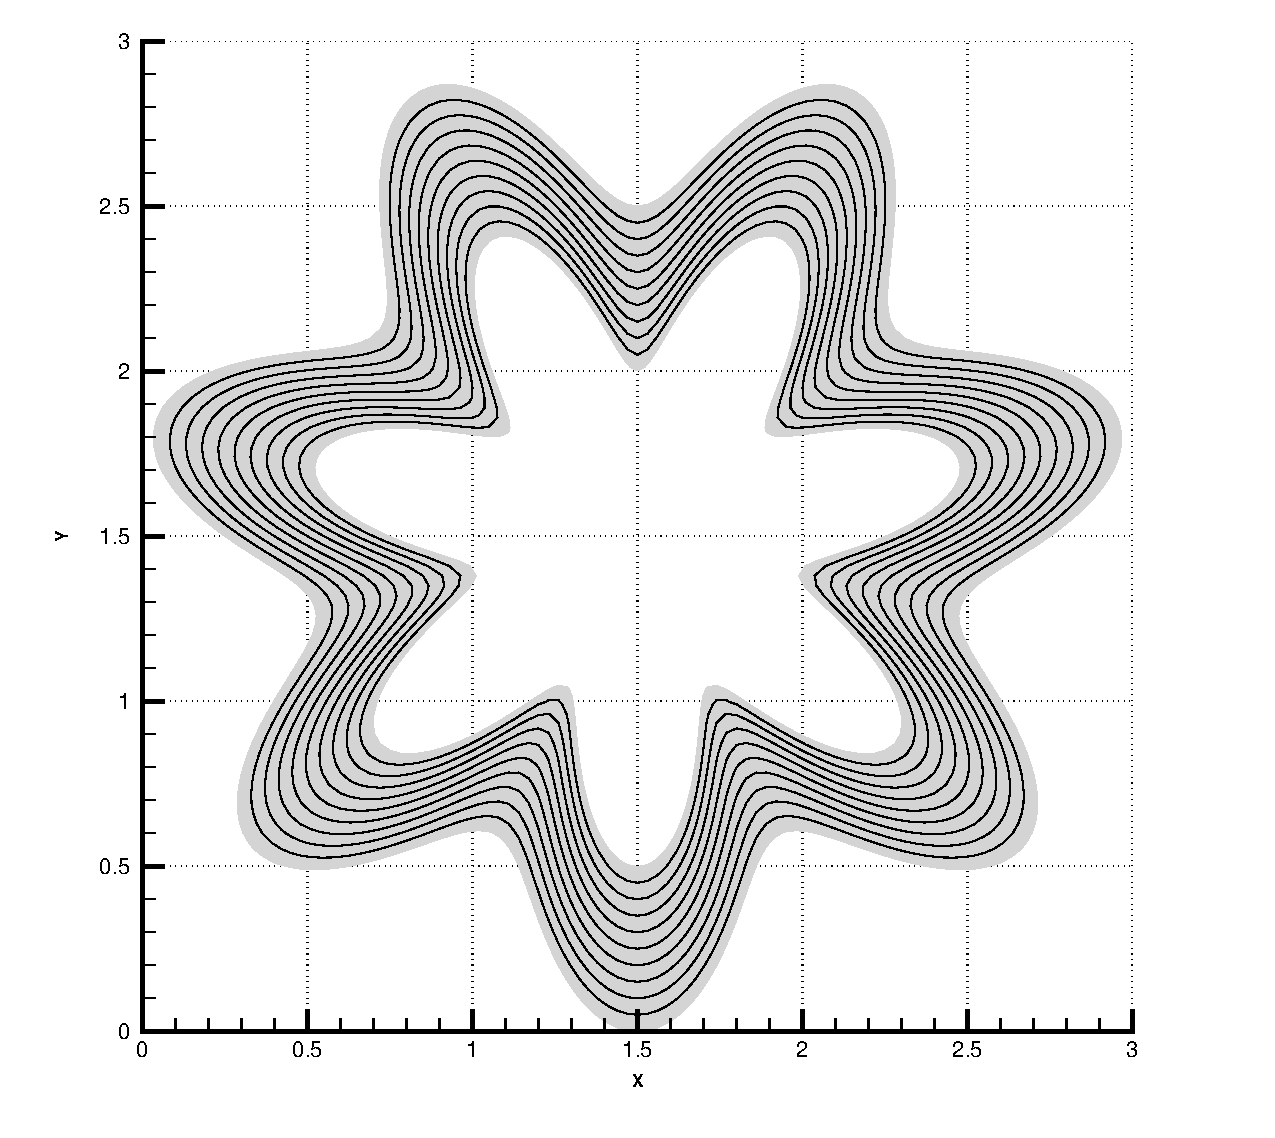
\includegraphics[width = 0.5\linewidth]{figs/waveyiso.eps} \label{fig:waveyisolines}} 
%%\subfloat[Isolines of exact solution at the initial and final time.]{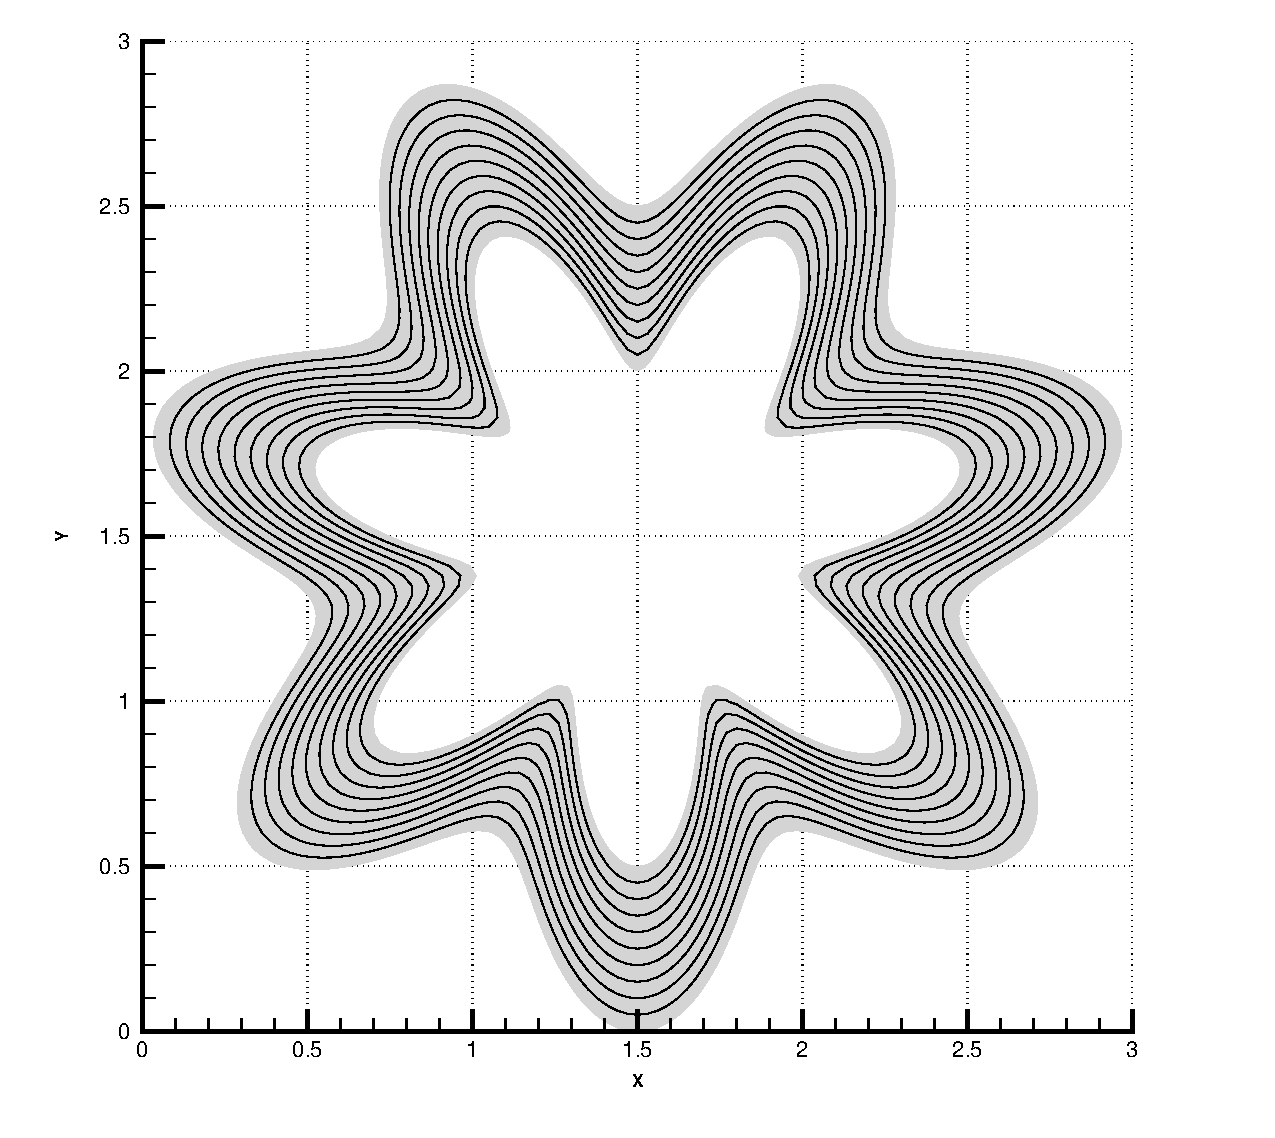
\includegraphics[width = 0.5\linewidth]{figs/waveyiso.eps} \label{fig:waveyisolines}} 
%%\quad
%\subfloat[Number of overlapping merging neighborhoods: one (blue), two (green), three (red).]{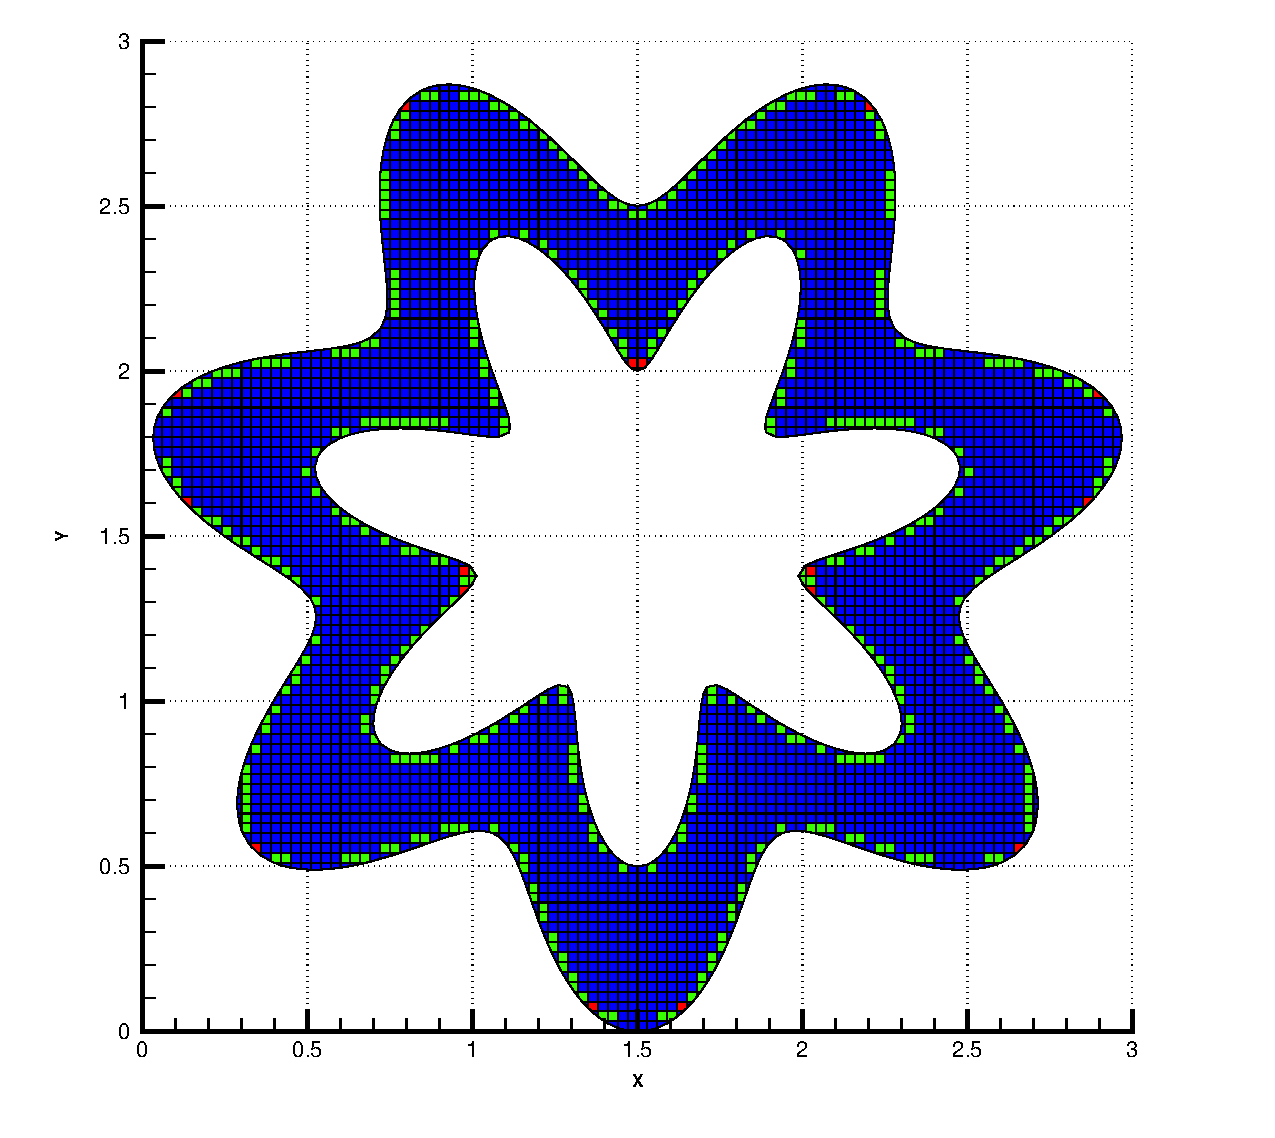
\includegraphics[width = 0.5\linewidth]{figs/waveynumhoods.eps}\label{fig:waveynumhoods}}
%% 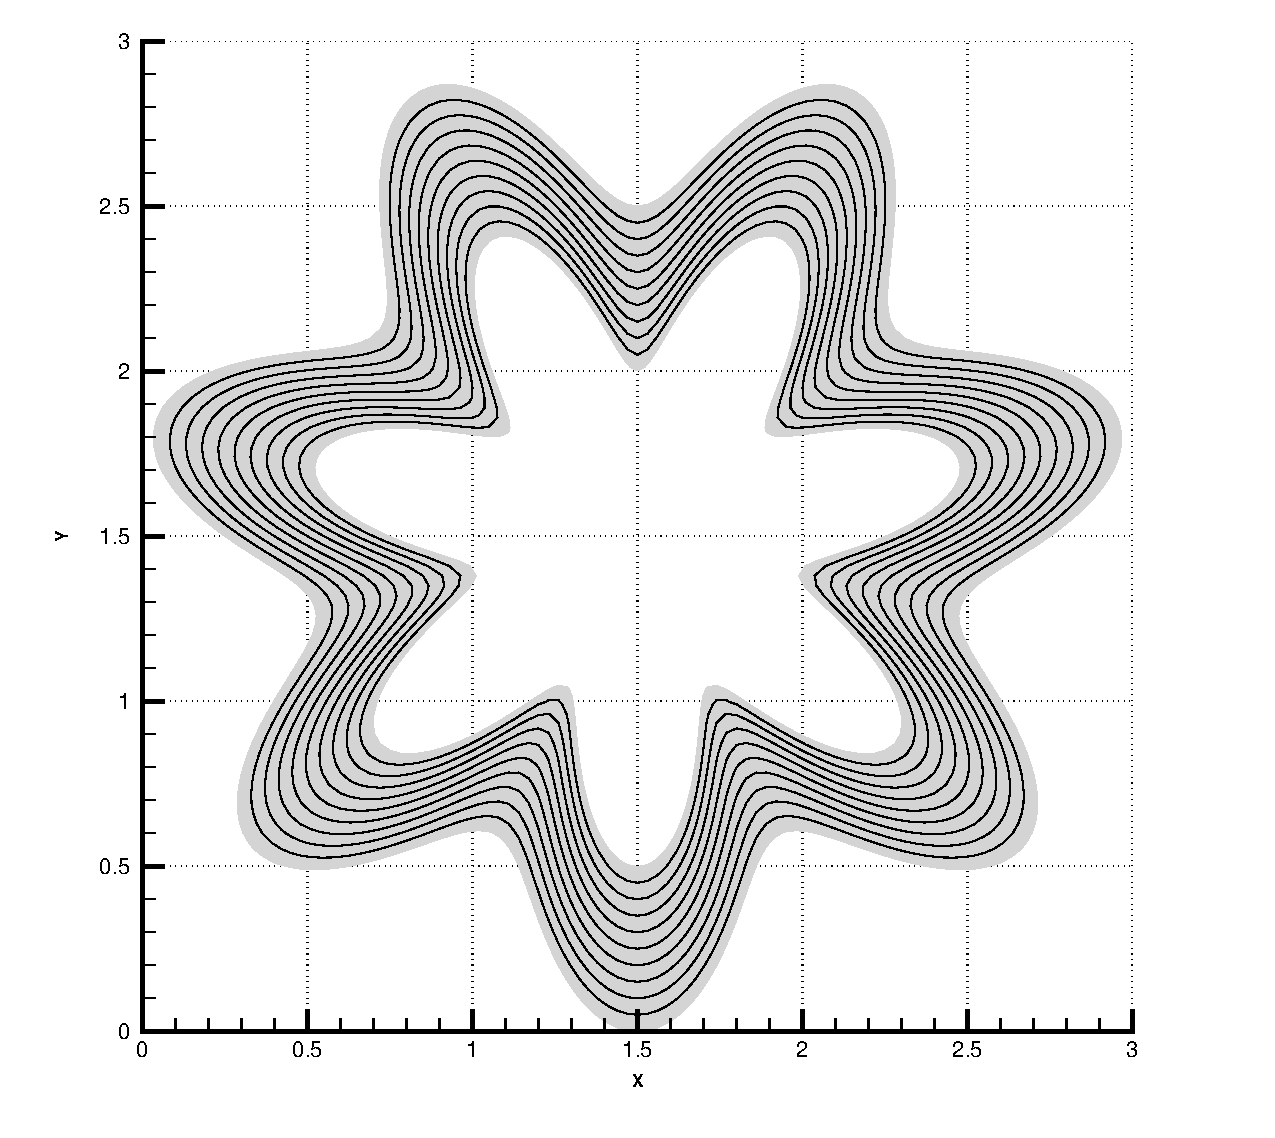
\includegraphics[width = 0.5\linewidth]{figs/waveyiso.eps} 
%\subfloat[Isolines of exact solution at the initial and final time.]{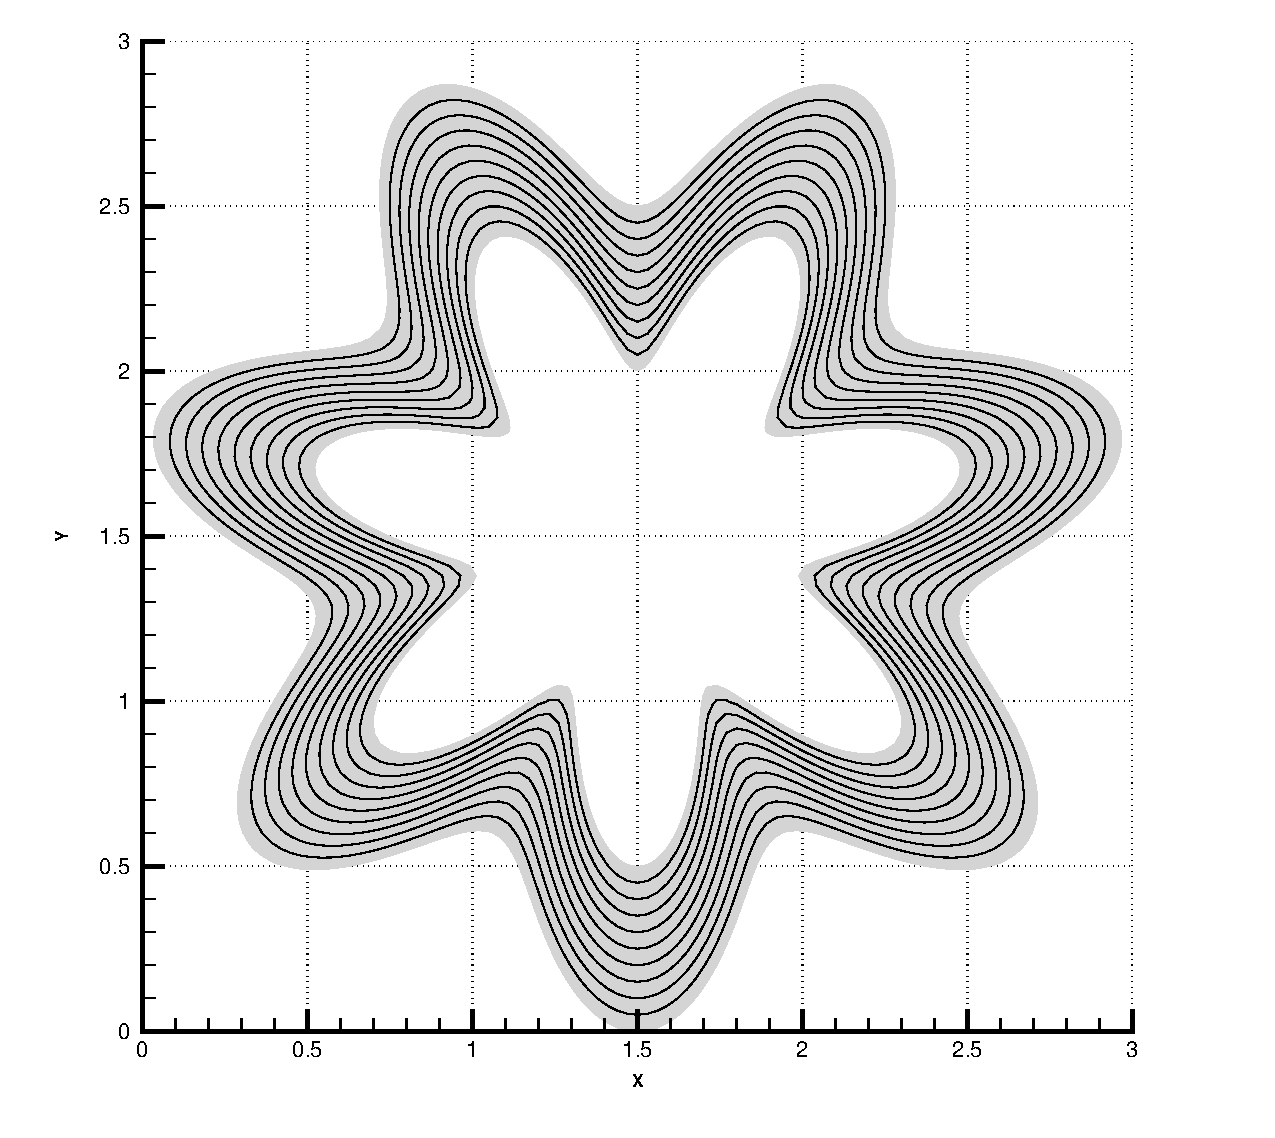
\includegraphics[width = 0.5\linewidth]{figs/waveyiso.eps} \label{fig:waveyisolines}} 
%\caption{Isolines of exact solution at the initial and final time for the
%wavy domain with overlapping neighborhoods. CANT SEE COLORS. WHAT DOES
%THIS EX ADD FROM PREVIOUS ONE} 
%% \label{fig:overlappingneighborhoods}
%% \label{fig:waveyisolines}} 
%\end{figure}
%
%In Figure \ref{fig:waveyisolines}, we show the isolines of the exact solution at the initial and final times.  Additionally, Figure \ref{fig:waveynumhoods} shows the number of overlapping neighborhoods on each cell.  In this example, we have at most three overlapping neighborhoods.  They are concentrated where the boundary has high curvature.   We do not observe growth in the numerical solution as indicated by $L_1$, $L_\infty$ errors of the solution at the final time listed in Table \ref{tab:overlappingerrors}.  Although this experiment does not prove stability of our numerical scheme, not observing unbounded growth in the numerical solution is a necessary condition.


\subsection{Supersonic vortex study}\label{sec:ssv}
We compute the solution to a supersonic flow 
around a quarter circle.  This problem has often been used in accuracy 
studies \cite{aftosmis:acc} since it has an exact solution to the Euler
equations that is smooth, given by 
\begin{equation}
\rho = \rho_i \left \{ 1 + \frac{\gamma-1}{2} \, M_i^2 \left [ 1 - (\frac{r_i}{r})^2
\right ] \right \} ^
{\frac{1}{\gamma-1}}
\end{equation}
and $ u = a_i \, M_i \, (\frac{r_i}{r})\,  \sin (\theta)$, 
$ v = a_i\,  M_i\,  (\frac{r_i}{r})\,  \cos(\theta)$, and
$ p = \rho^\gamma / \gamma$.
Here, the inner radius is $r_i = 1.0$,  the outer radius
is $r = 1.384$, $\rho_i=1$, and the Mach number on the inner circle
$M_i = 2.25$ in our experiments. 
In this
normalization we use $a_i = 1$, $p_i = 1/\gamma$. 
The second order MOL scheme is used, and we march
to steady state, until the maximum density update is below $10^{-10}$.  
The solution is smooth, so no limiters are needed.
The exact solution is used to set the ghost cells at the inflow and
outflow boundaries. The domain size is 1.43 by 1.4301 (slightly different
to prevent mesh  degeneracies).  

In Table \ref{tab:ssv} we compare the accuracy of three different formulations
for the cut cell gradients. 
For first order accurate gradients, we use a linear least squares reconstruction for
both the irregular cell gradient (cut cells and their one-away neighbors) 
described in Section \ref{sec:limit}, and the SRD gradients, which 
update the cut cell solution after stabilization. Second order accurate 
gradients fit a quadratic for both
the cut cells and tiles as described in Section \ref{sec:limit}, 
but only the first derivative terms are used. 
As an intermediate experiment, we  fit a quadratic using least squares but treating the
cell averages as pointwise values at the cell centers. Here again
the second derivative terms are ignored.  Note that this is not
second order accurate, since the centroid value differs by $O(h^2)$
from the pointwise value at the centroid. Nevertheless, this is frequently
done since it is easier to implement, in particular for the SRD neighborhoods
with irregular shapes. 



{
\small
\begin{table}[h]
\centering
	\hspace*{-.3in}
	\subfloat[$L_1$ volume errors. \label{tab:ex1_L1vol}]{
		\begin{tabular}{|l|c|l|l|l|}
			\hline
			$h$ & $N_x, N_y$ & 1st order grad. & ptwise grad. & 2nd order grad.   \\
			\hline
			.5297 & 27 & 6.75e-3 & 2.76e-3 & 2.45e-3 \\
			\hline
			.2648 & 54  & 1.78e-4 (3.8)  & 6.38e-4 (4.3) & 4.71e-4 (5.2) \\
			\hline
			.1324 &108 & 3.63e-4 (4.9)  & 1.53e-4 (4.2) & 1.21e-4 (3.9) \\
			\hline
			.662e-2 & 216 & 6.52e-5 (5.6)  & 3.65e-5  (4.2) & 2.98e-5 (4.1) \\
			\hline
			.331e-2 & 432 & 1.40e-5 (4.7)  & 8.85e-6  (4.1) & 7.86e-6 (3.8) \\
			\hline
			.166e-2 & 864 & 2.68e-6 (5.2)  & 2.15e-6  (4.1) & 2.04e-6 (3.9) \\
			\hline \hline
		\end{tabular}
	}
	\quad
	\vspace*{.2in}
	
	\hspace*{-.3in}
	\subfloat[$L_1$ boundary errors. \label{tab:ex1_L1bndry}]{
		\begin{tabular}{|l|c|l|l|l|l|}
			\hline
	    $h$ &  $N_x, N_y$   & 1st order grad.  & ptwise grad. &  2nd order grad.    \\
	\hline
     .5297 & 	27  &   6.84e-02 &  3.31e-02  & 2.37e-2\\
	\hline
     .2648 &	54  &   2.83e-02 (2.4) &  1.21e-02 (2.7)  & 8.183-3  (2.9) \\
	\hline
      .1324 &	108 &   1.03e-02  (2.8)&  4.69e-03 (2.6) & 3.453-3 (2.4) \\
	\hline
     .662e-2 &	216 &   3.65e-03  (2.8) &  1.82e-03 (2.6) & 1.38e-3 (2.5) \\
			\hline
    .331e-2 &	432 &   1.24e-03  (3.0)  &  7.18e-04 (2.6) & 6.15e-4 (2.2) \\
			\hline
    .166e-2 &	864 &   3.96e-04  (3.1)  &  2.85e-04 (2.6) & 2.58e-4 (2.4) \\
			\hline \hline
		\end{tabular}
	}
	
	\caption{\sf L1 norm of the error in the domain volume and along the boundary,
        for the supersonic vortex example. The error using first order accurate
        gradients, pointwise quadratic, and fully second order accurate gradients is shown. 
        Pointwise quadratic gradients have half of the error than first order gradients. 
        Truly second order accurate gradients are even better, especially on coarser grids. \label{tab:ssv}}
\end{table}
}

We measure the $L_1$ norm of the error in the volume,   $\sum_{i,j} \,
V_{ij} \lvert e_{ij } \rvert$ and at the boundary, $ \sum_{{i,j} \in \partial \Omega} \, A_{ij} \lvert e_{ij
} \rvert$.  Here
$e_{i,j}$ is the error at the cell centroid, and $A_{ij}$ is the length of the 
boundary segment in cut cell $(i,j)$.
These are given in Table \ref{tab:ex1_L1vol} and \ref{tab:ex1_L1bndry}. 
For easier comparison with other papers we also give the mesh size 
to a few digits. In  a cut cell mesh there are both solid and
flow cells, so the total number of cell is larger than the number of
flow cells, and not as easy to compare as the mesh spacing.
All interior cells use the evolution scheme and gradients, so
the difference in the errors are solely due to the cut cell gradients.

\begin{figure}[h]
	\begin{center}
		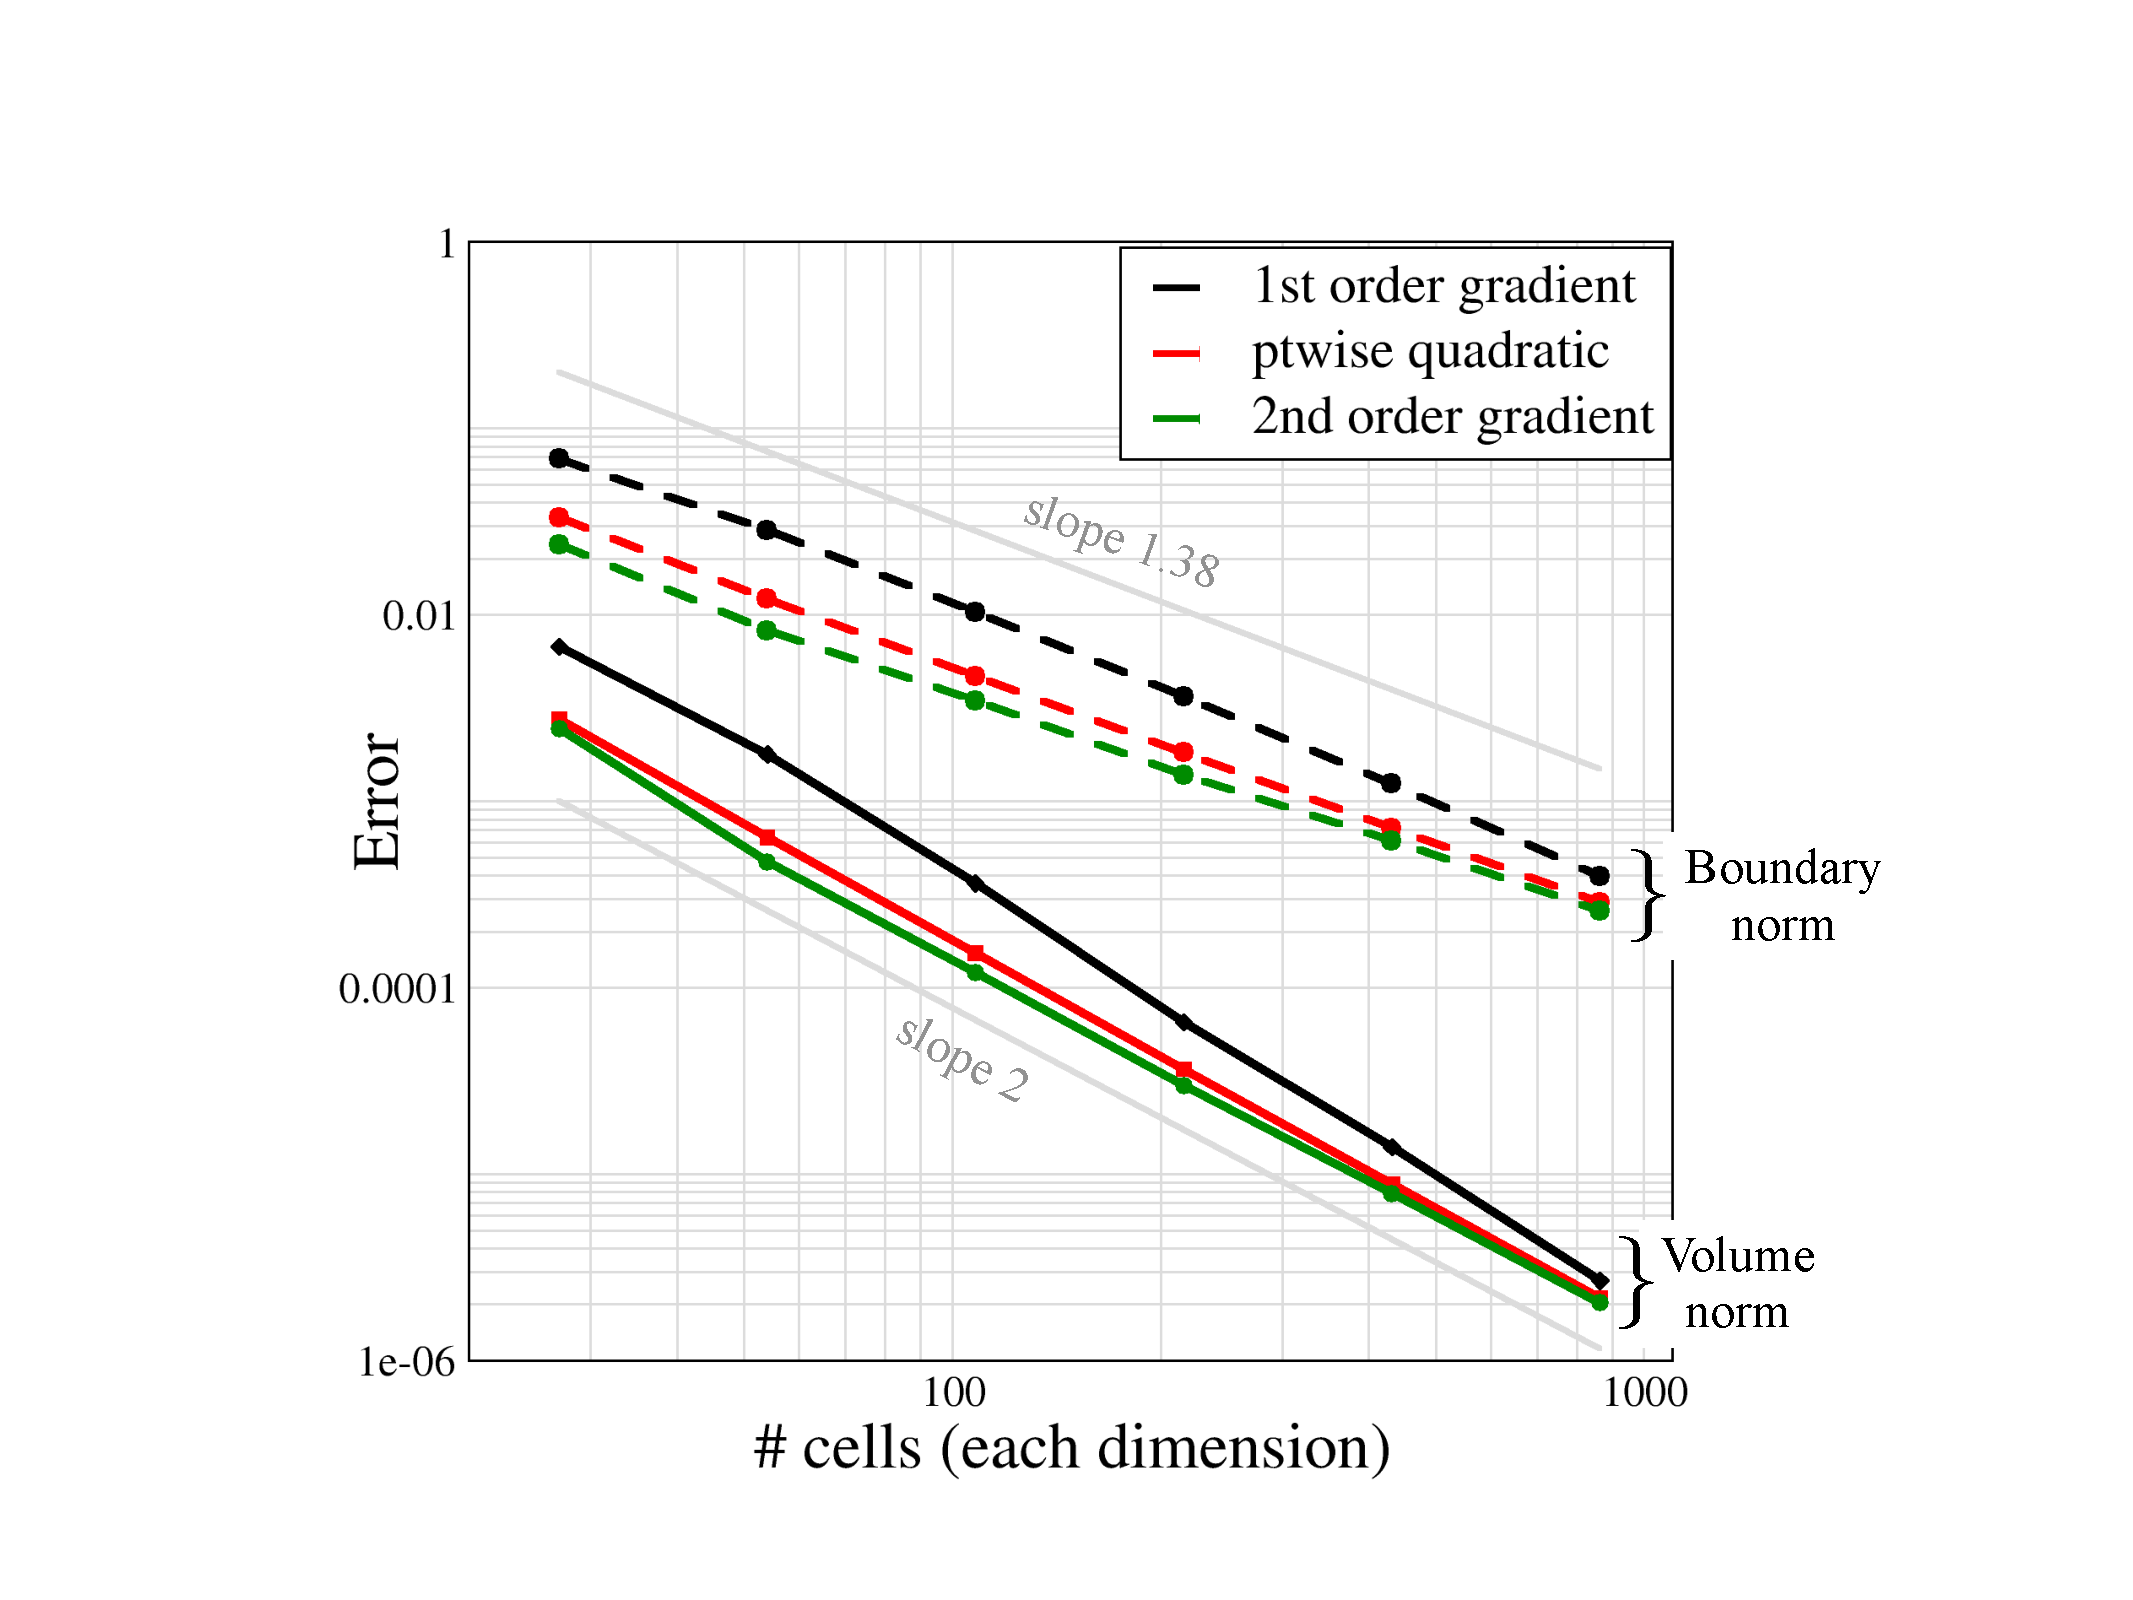
\includegraphics[height=3.0in]{figs/gradientConv.pdf}
		\caption{\sf Convergence in the L1 norm of the error in the entire 
			domain  (solid line), and along the boundary (dashed line).
			The reference line has slope 2 next to the domain error. The convergence
			rate at the boundary is between 1.38 and 1.5
			along the boundary.
			\label{fig:ssv}}
	\end{center}
\end{figure}


Note that the error at the cut cells is larger than in the volume, and has a
slower convergence rate. Since the number of cut cells grows only
linearly with refinement, the $L_1$
accuracy in the entire flow field is still second order.  At the boundary,
Richardson extrapolation shows that the convergence rate seems to be
between 1.38 and 1.5.
This has also been found in other cut cell studies \cite{KB:2006,nemec_tm14}, and 
is not due to SRD.

Figure \ref{fig:ssv} and Table \ref{tab:ssv}  show that using pointwise 
quadratic cut cell gradients is roughly
a factor of 2 more accurate on coarser grids.  The more complicated second order
acccurate gradient is even more accurate, especially on coarser grids.  Ultimately the gradient
error is reduced, and the error curves for the first and second order 
accurate gradients approach each other. 


We also use this example to compare the effect of state redistribution versus 
marching to steady state using local time-stepping without SRD.  
Table  \ref{tab:ssv2} shows a comparison of the error in the converged
solution using local time stepping (LTS)  without SRD, and the error with full timesteps and
SRD stabilization, both using  first order accurate gradients. 
The errors are essentially identical, showing that 
SRD does not degrade the computed solution with too much diffusion due
to the merging neighborhoods. This holds across all the other
gradient formulations too.


{
\small
\begin{table}[h]
\centering
 	\begin{tabular}{|l|c|l|l||l|l|} \hline
 		$h$ & $N_x ,N_y$ & \multicolumn{2}{|c|} {Volume Error} & \multicolumn{2}{|c|}{Boundary Error} \\ 
                \hline
 		    &            & {LTS (no SRD)} & SRD  & LTS (no SRD)  & SRD  \\ \hline
 			.5297 & 27 & 6.09e-3  &  6.75e-3   &  6.75e-02       &  6.84e-02 \\
 			\hline
 			.2648 & 54  & 1.67e-3  (3.6)  & 1.78e-4 (3.8)  &  2.79e-02  (2.4) &  2.83e-02 (2.4) \\
 			\hline
 			.1324 &108 & 3.41e-3  (4.9)  & 3.63e-4 (4.9)   &  1.00e-02  (2.8) &  1.03e-02  (2.8)\\
 			\hline
 			.662e-2 & 216 & 6.62e-5  (5.2)  & 6.52e-5 (5.6)  &  3.51e-03  (2.9) &  3.65e-03  (2.8)\\
 			\hline
 			.331e-2 & 432 & 1.34e-5  (4.9)  & 1.40e-5 (4.7)  &  1.21e-03  (2.9) &  1.24e-03  (3.0)  \\
 			\hline
 			.166e-2 & 864 & 2.59e-6  (5.2)  & 2.68e-6 (5.2)  &  3.78e-04  (3.2) &  3.96e-04  (3.1)  \\
 			\hline \hline
 	\end{tabular}
 	\caption{\sf Comparison of errors using local time stepping, which does not use SRD, 
        and regular time stepping with SRD. (The SRD errors are repeated here for easier
        comparison.) The errors are almost identical, except on the coarsest
        grid, showing that SRD does not 
        degrade the solution with too much diffusion. \label{tab:ssv2}}
\end{table}
}



\subsection{Shock Reflection from  Cylinder}
Next we demonstrate the method for the Euler equations using a Mach 2
shock diffracting around a circular cylinder. A cylinder with radius $0.15$ is centered at
(0.5,0.5), and the shock is initially located at $x = 0.2$.
For this example we compare results using the MUSCL scheme and
the Method of Lines as the base schemes, both using local Lax Friedrichs for the Riemann
solver. The BJ limiter is used to limit
both the base scheme irregular cells  and tile reconstruction gradients. 

Figure \ref{fig:cyl1} (left) shows the solution density from MUSCL, and
right from MOL, at time $t=0.25$. 
Both grids use 302 cells in each
directions, and the domain is  $[0.0,0.0,]$ by  $[1.00001, 1.0]$, again to
prevent mesh degeneracies.
There are 416 cut cells
around the cylinder; 160 of the cut cells had volume fractions less than
0.5 and were stabilized with SRD.  The smallest volume fraction was 1.17E-4.   
For comparison, this is also the time shown in \cite{mjb-hel-rjl:hbox2}. 
Here and in \cite{mjb-hel-rjl:hbox2}, the front of the cylinder where the
maximum density is found is better behaved with the one-step methods than with
MOL.  The method of lines solution is smoother around the boundary than our
MUSCL variant (see Figure \ref{fig:cylbndry}).

\begin{figure}[h]
\begin{center}
\vspace*{-.1in}
\hspace*{-.4in}
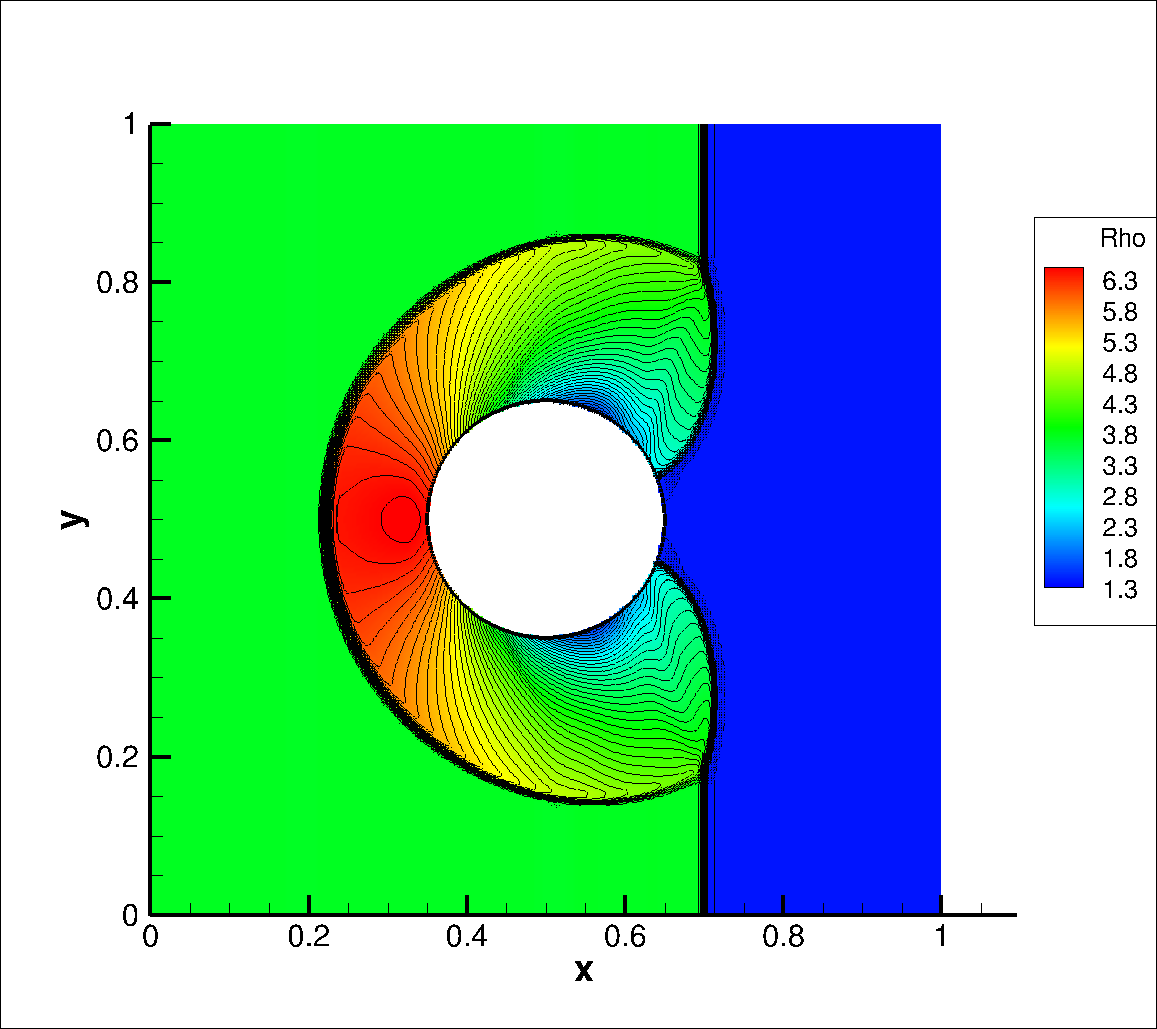
\includegraphics[width=0.48\linewidth,trim=10 10 200 10,clip]{figs/muscl_302cells.png}
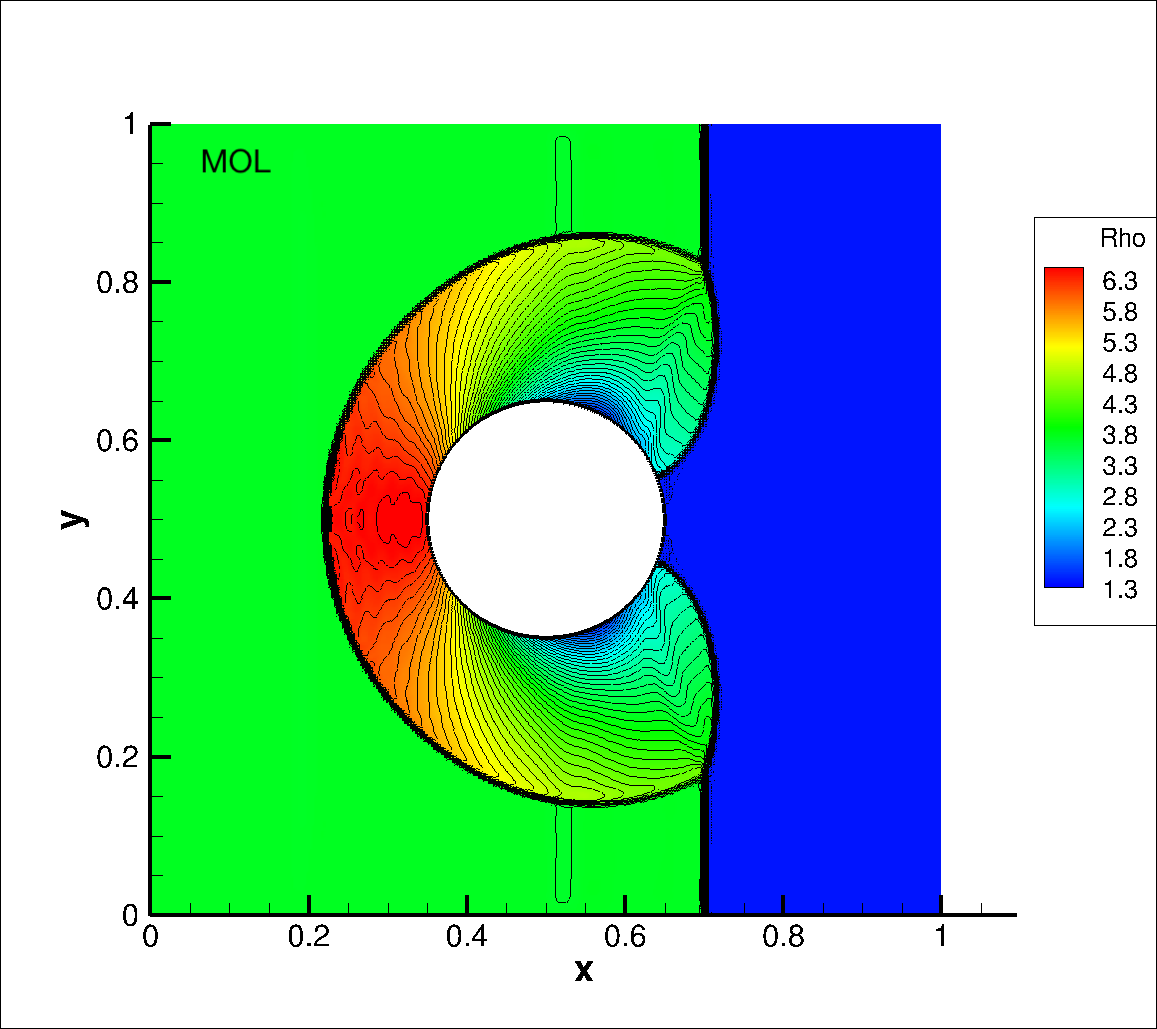
\includegraphics[width=0.48\linewidth,trim=10 10 200 10,clip]{figs/MOL_302cells.png}
\caption{\sf Density profile of Mach 2 shock reflection around a cylinder,
at time t=0.25.  Left computation used MUSCL, right used MOL. 
There are 52 contours between 1.3 and 6.5.
The front of the cylinder is better behaved with MUSCL, but the solution
at the cut cells is better  with the method of lines.
\label{fig:cyl1}}
\end{center}
\vspace*{-.1in}
\end{figure}

Figure \ref{fig:cylbndry}
shows the density profile from both schemes
taken along the cylinder.
For this plot, the cut cell variable is
reconstructed to the midpoint of the cylinder line segment in each  cell.  
The zoom shows the difference more
clearly.

\begin{figure}
\begin{center}
%\includegraphics[width=0.48\linewidth,trim=20 20 20 30,clip]{figs/densityCompare_302_normalvs3by3.png}
\hspace*{-.5in}
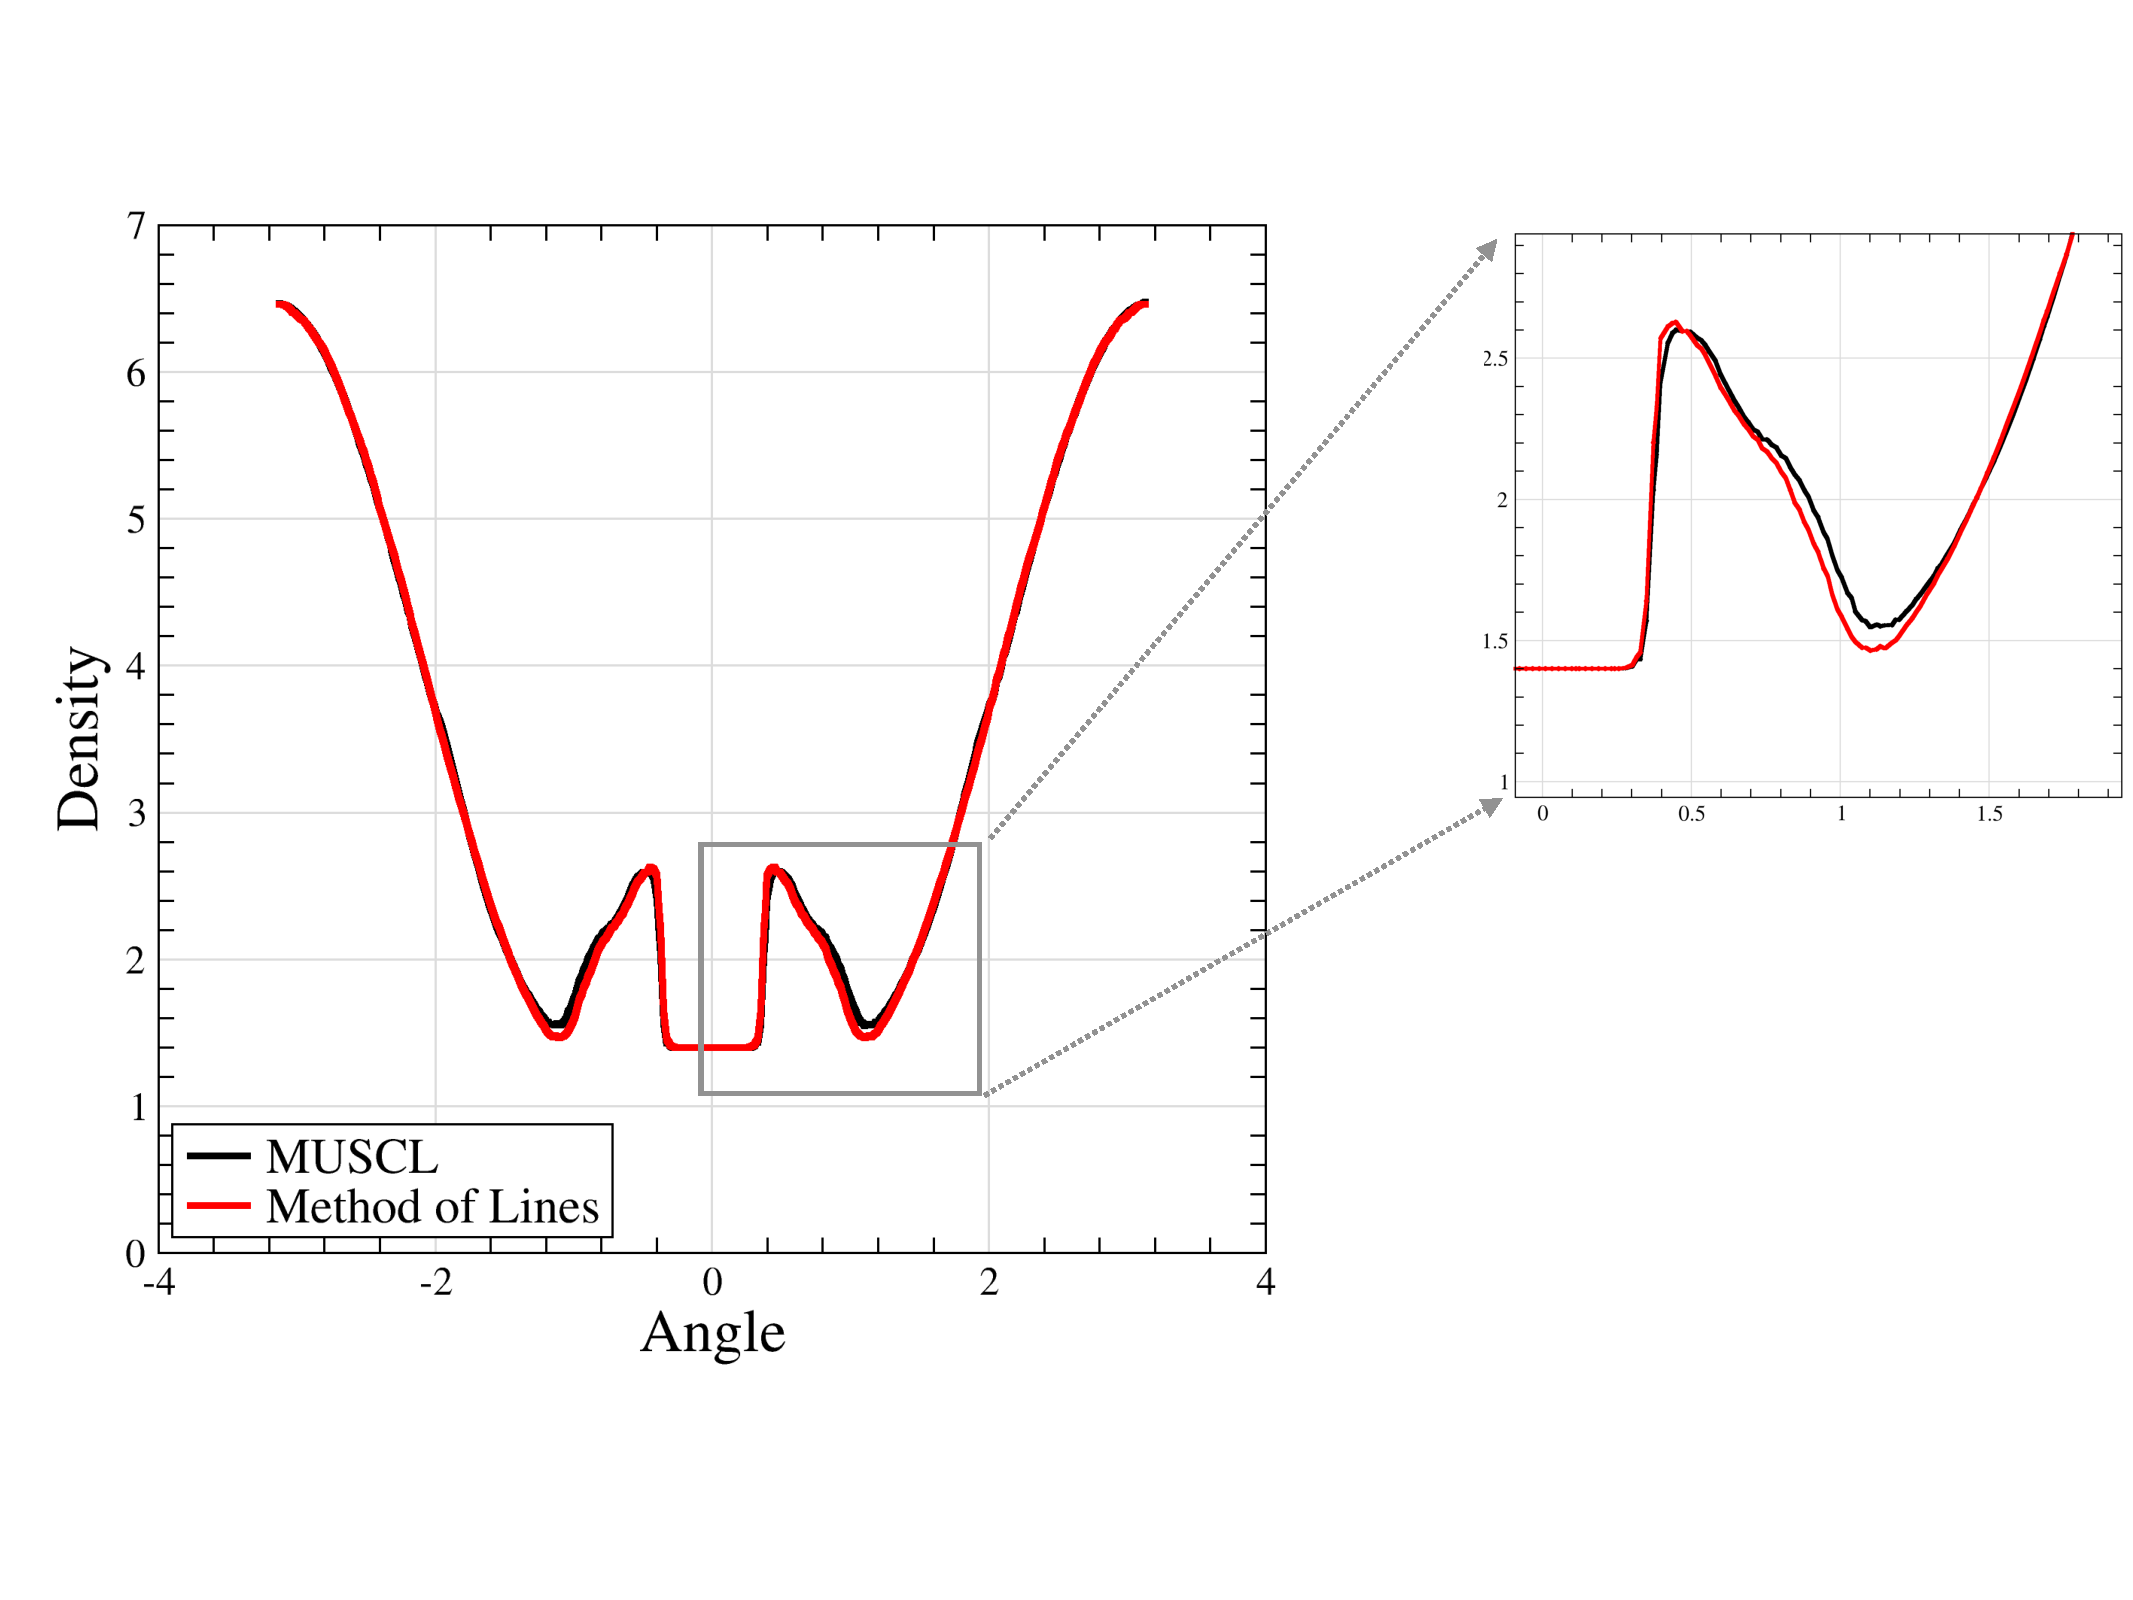
\includegraphics[height=2.7in]{figs/MM_densityBndry.pdf}
\hspace*{.3in}
%\includegraphics[width=0.48\linewidth,trim=20 20 20 30,clip]{figs/pressureCompare_302_normalvs3by3.png}
%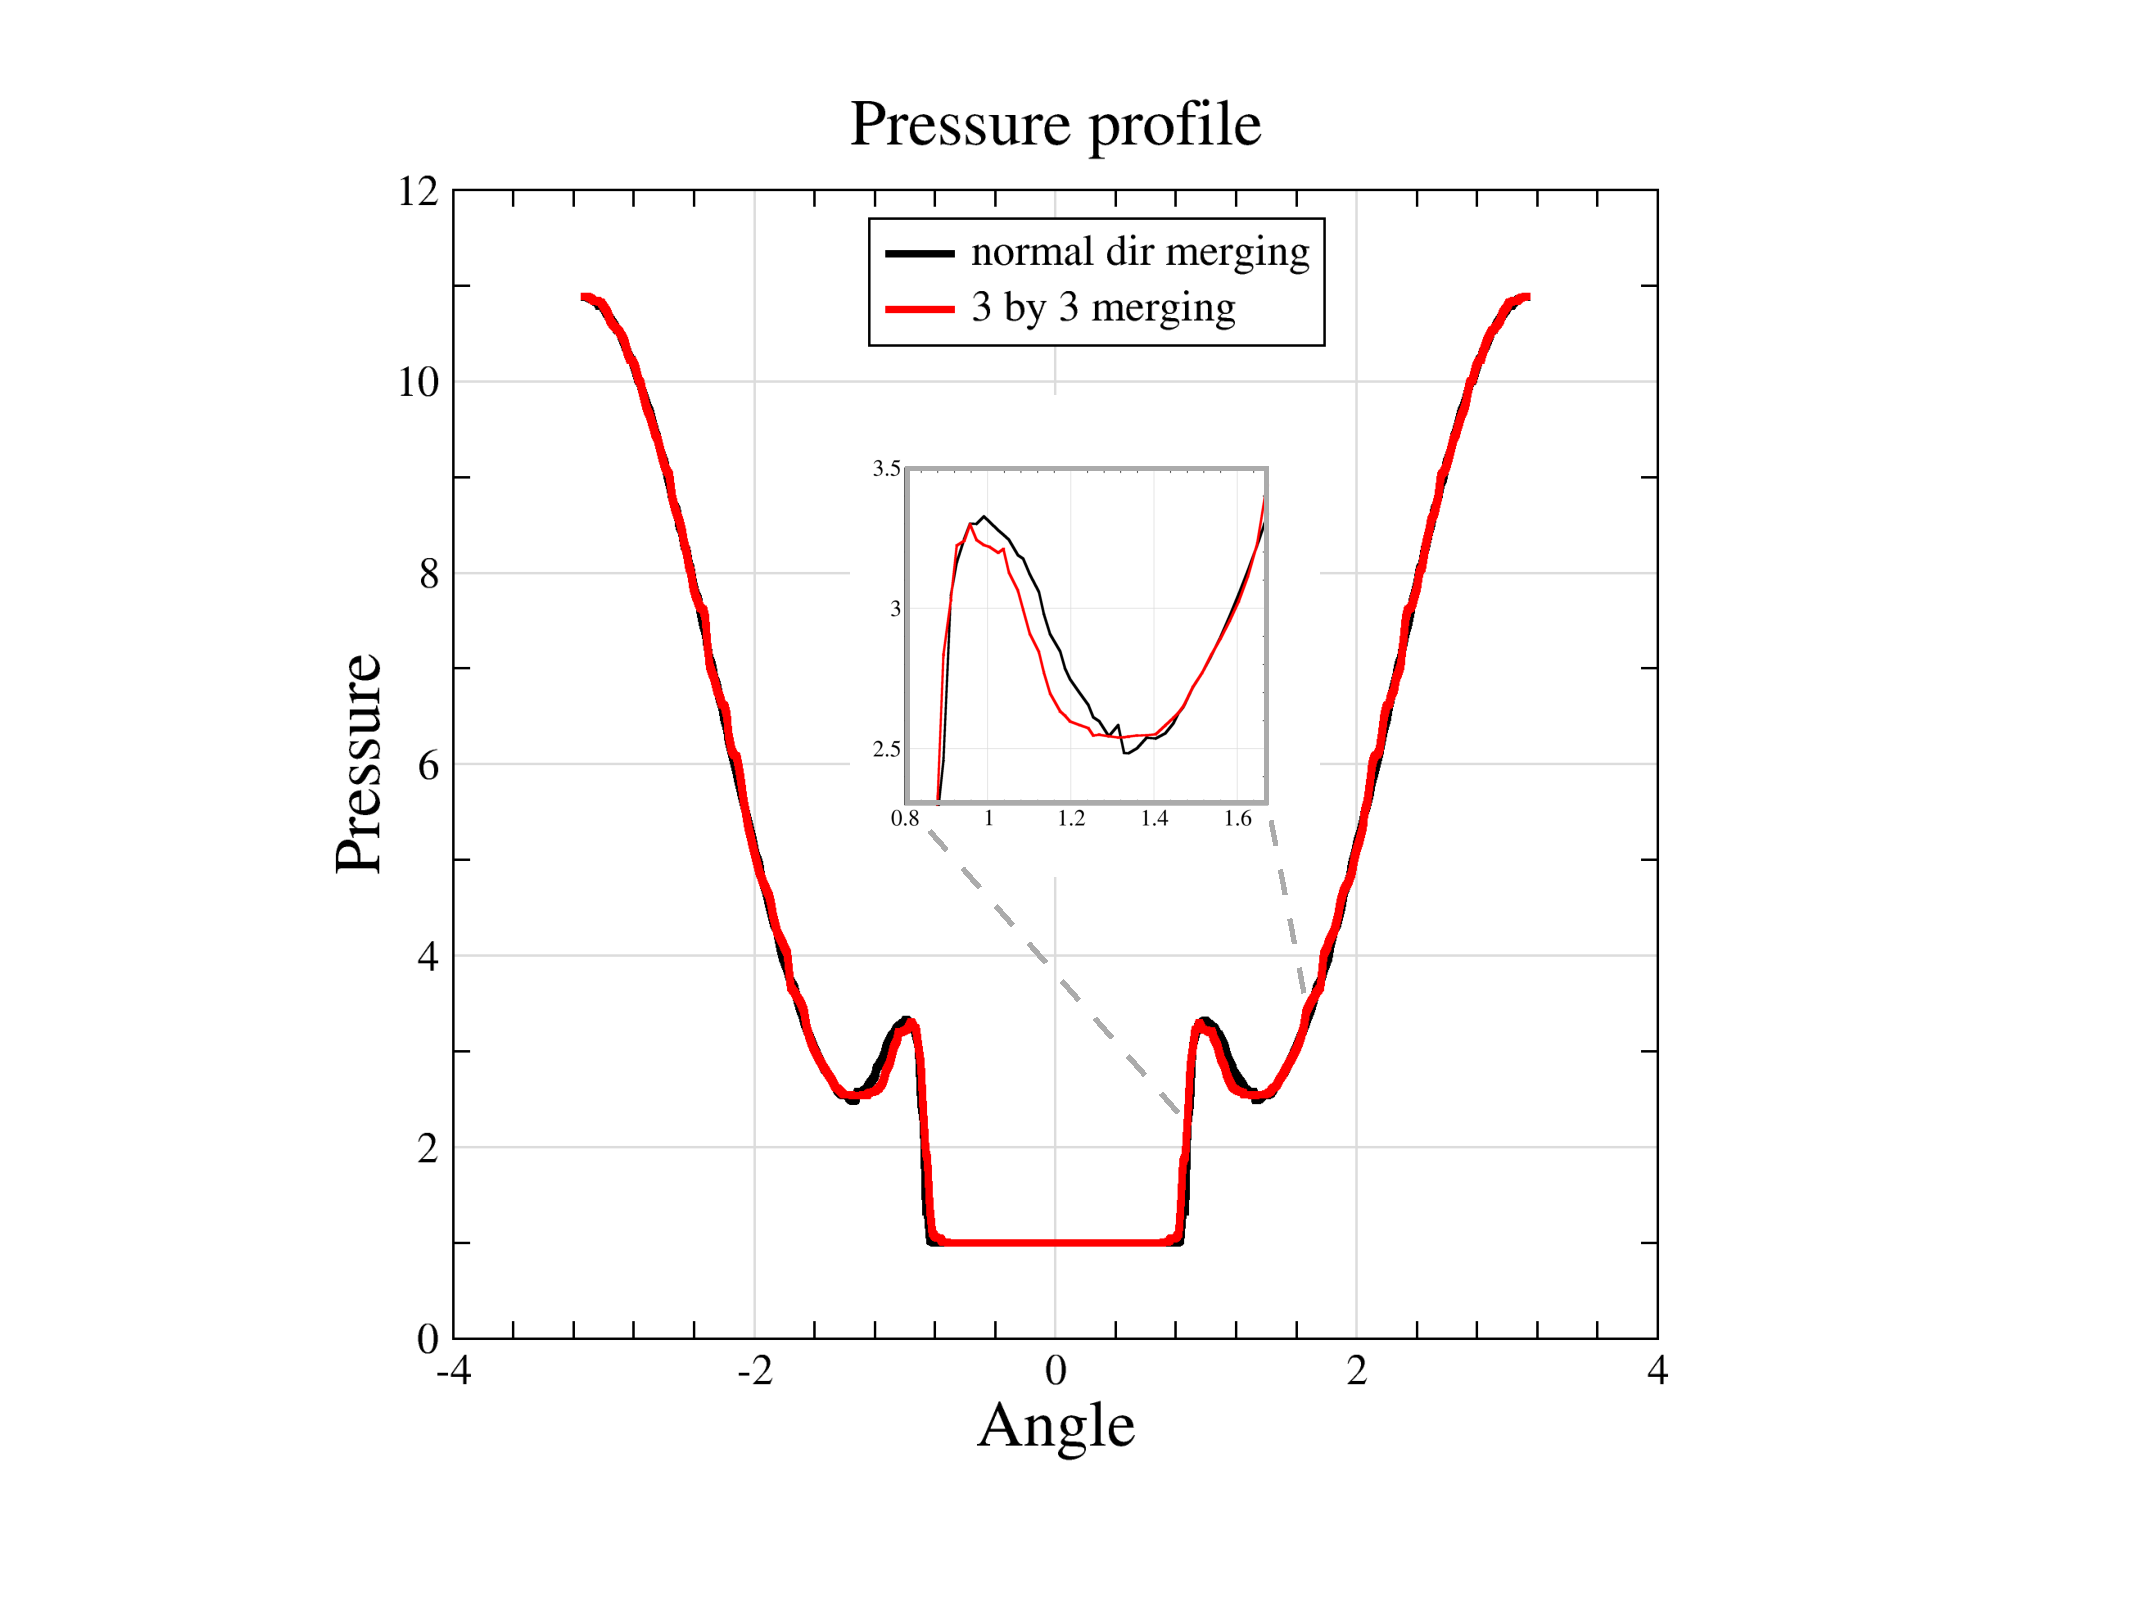
\includegraphics[height=2.7in,trim=120 70 230 50,clip]{figs/pressureWithZoom.pdf}
\caption{\sf The density profile  around the cylinder for the MUSCL and MOL schemes 
at time t=0.25.  The MOL scheme has smoother results.}
\label{fig:cylbndry}
\end{center}
% fig in amrclaw-amrcart/example/cylinder_Mach2 directory on juniper
% using sortedcyl.dat (coied from bndry01.dat) in the various _output dirs
\end{figure}

\clearpage

\subsection{Double Mach Reflection problem}\label{sec:dm}
In this section, we reflect a Mach 10 shock obliquely over a wedge, 
where the shock and wall form a $60^{\circ}$ angle.  
The problem domain is $[0,3.0]\times[0,1.75]$, with an angled wall 
passing through the point $(1/6,0)$ . The ramp is outlined in red in Figure
\ref{fig:dm}.
We use the finite volume MUSCL scheme with second order slopes on the base 
grid and SRD neighborhoods, and limit using Barth Jespersen.
The solution to this problem is a complex, self-similar reflection pattern 
composed of incident and reflected shocks, Mach stem, and a contact 
discontinuity \cite{WOODWARD1984115,rkdg5}.  
The contact discontinuity is an unstable feature of the solution that can be 
difficult to resolve correctly, especially in the neighborhood of the 
reflecting boundary where the carbuncle phenomenon can occur \cite{KEMM2018596}.

\begin{figure}[h]
\centering
%\includegraphics[width=0.48\linewidth]{figs/doublemach.png}
%\includegraphics[width=0.48\linewidth]{figs/doublemach_zoom.png}
%\includegraphics[width=1.1\linewidth]{figs/doubleMach.pdf}
\hspace*{-.25in}
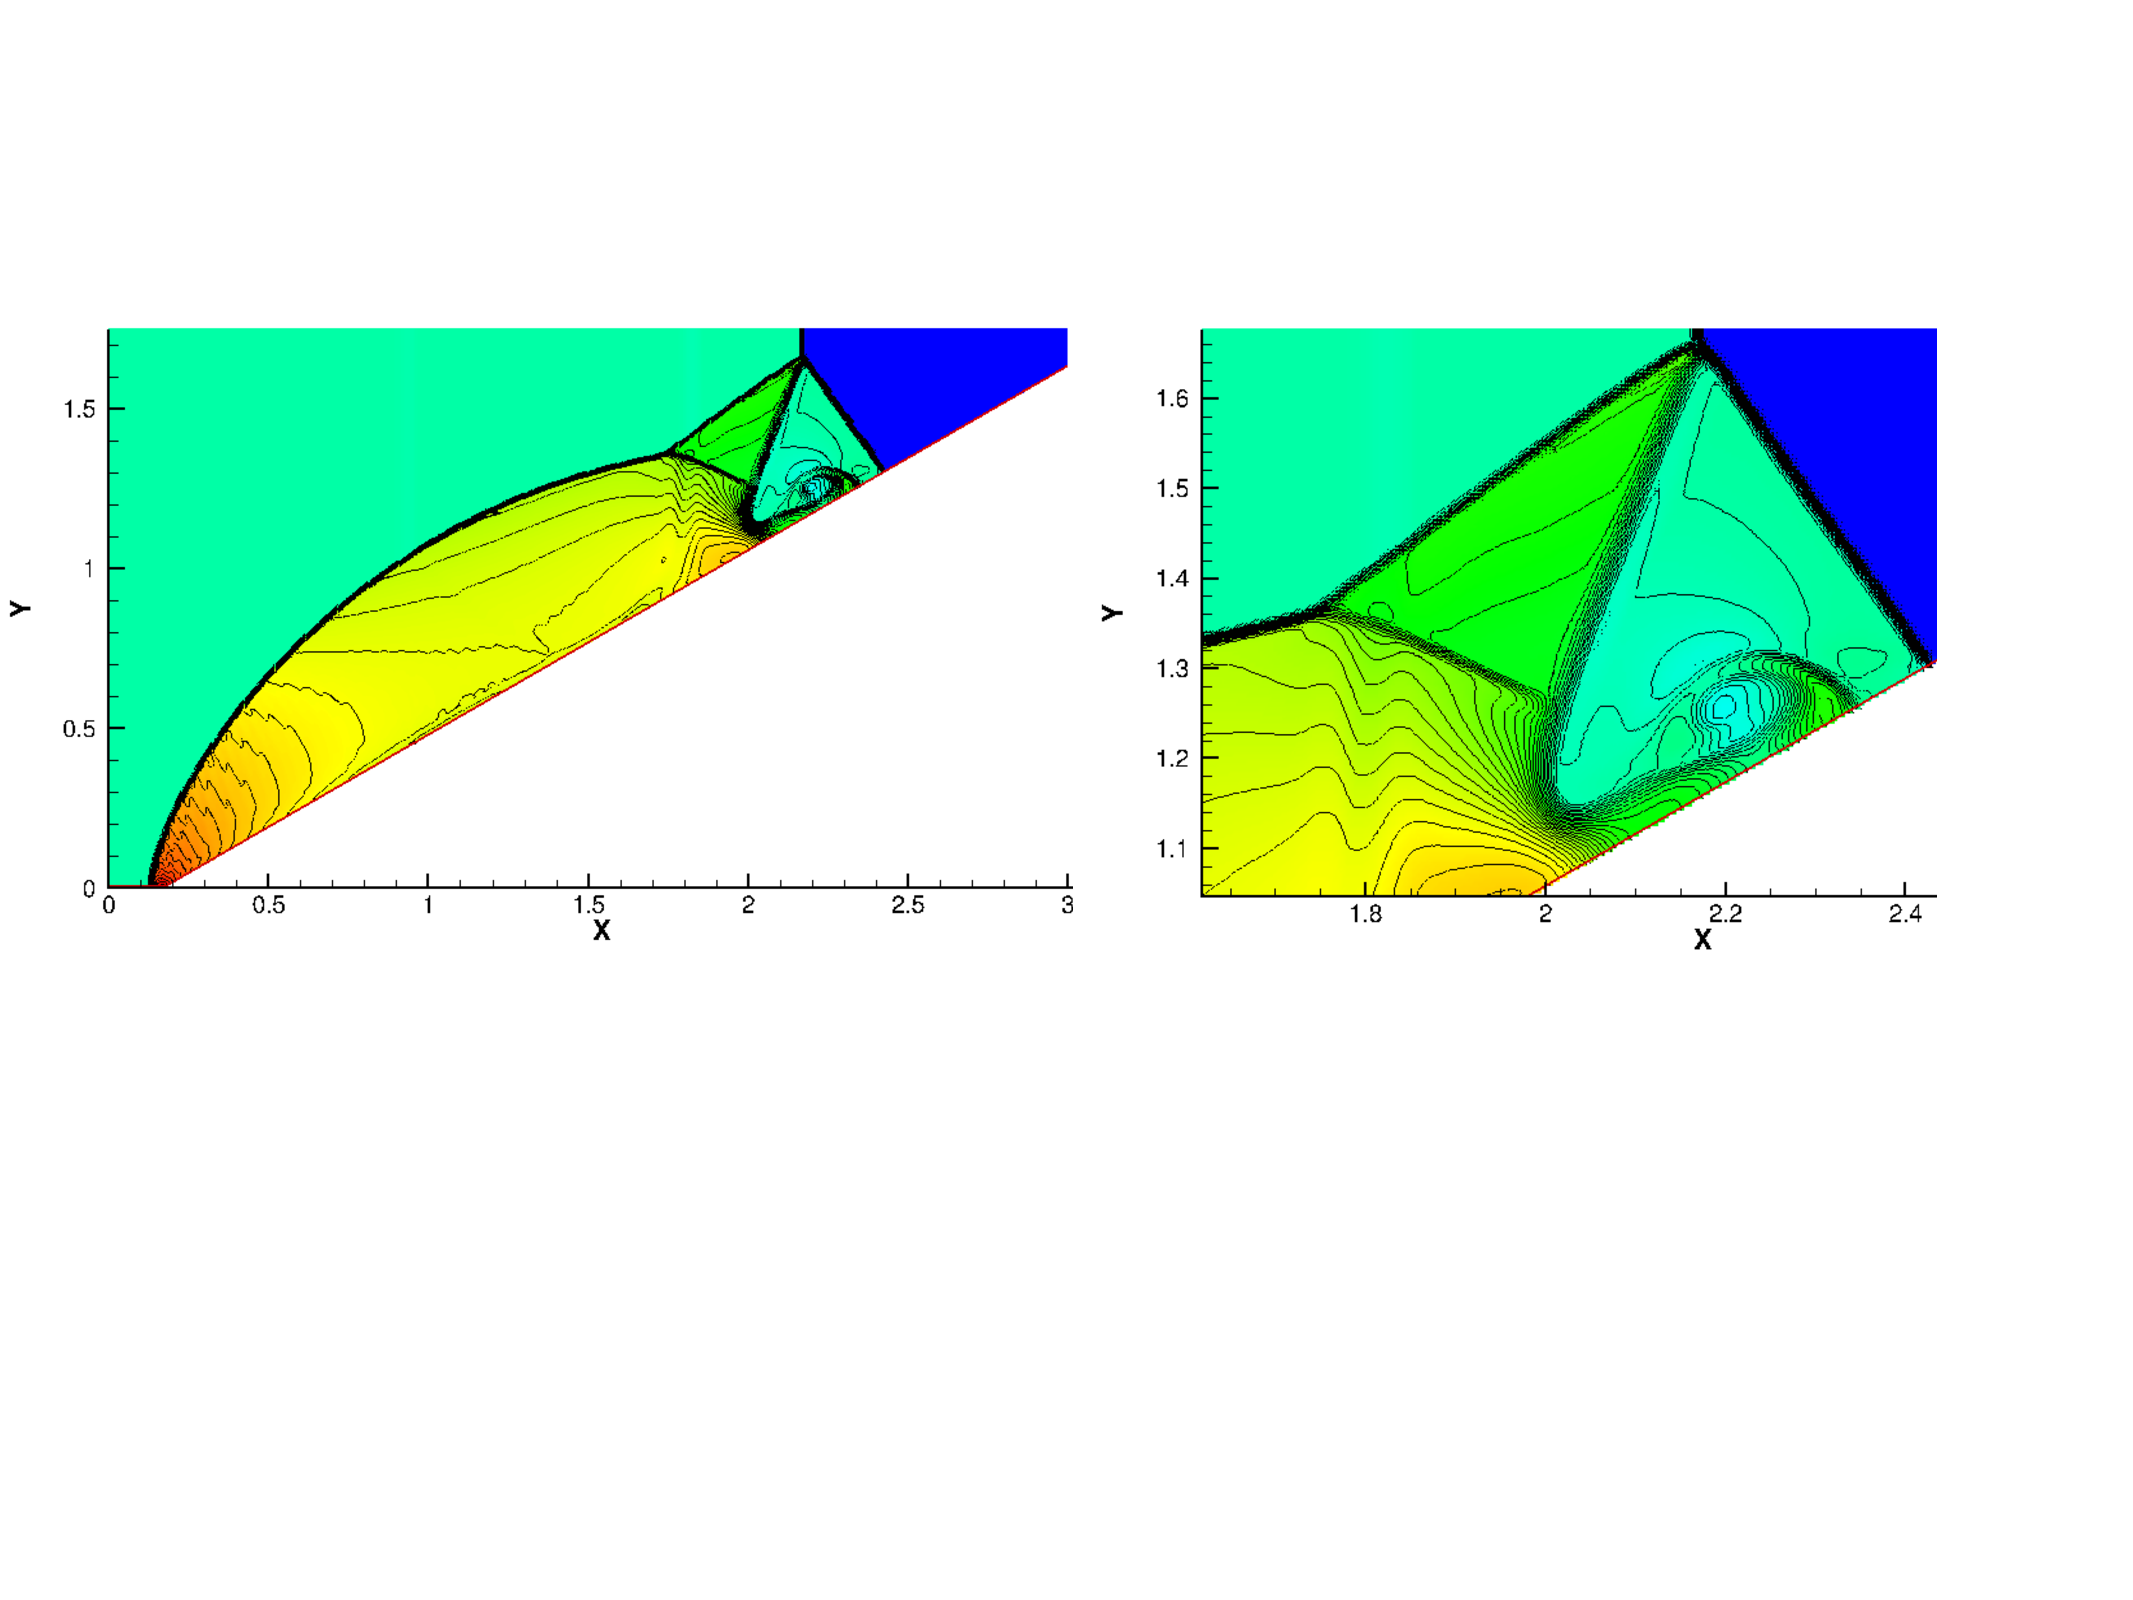
\includegraphics[width=1.1\linewidth]{figs/doubleMach240.pdf}
\hspace*{-.25in}
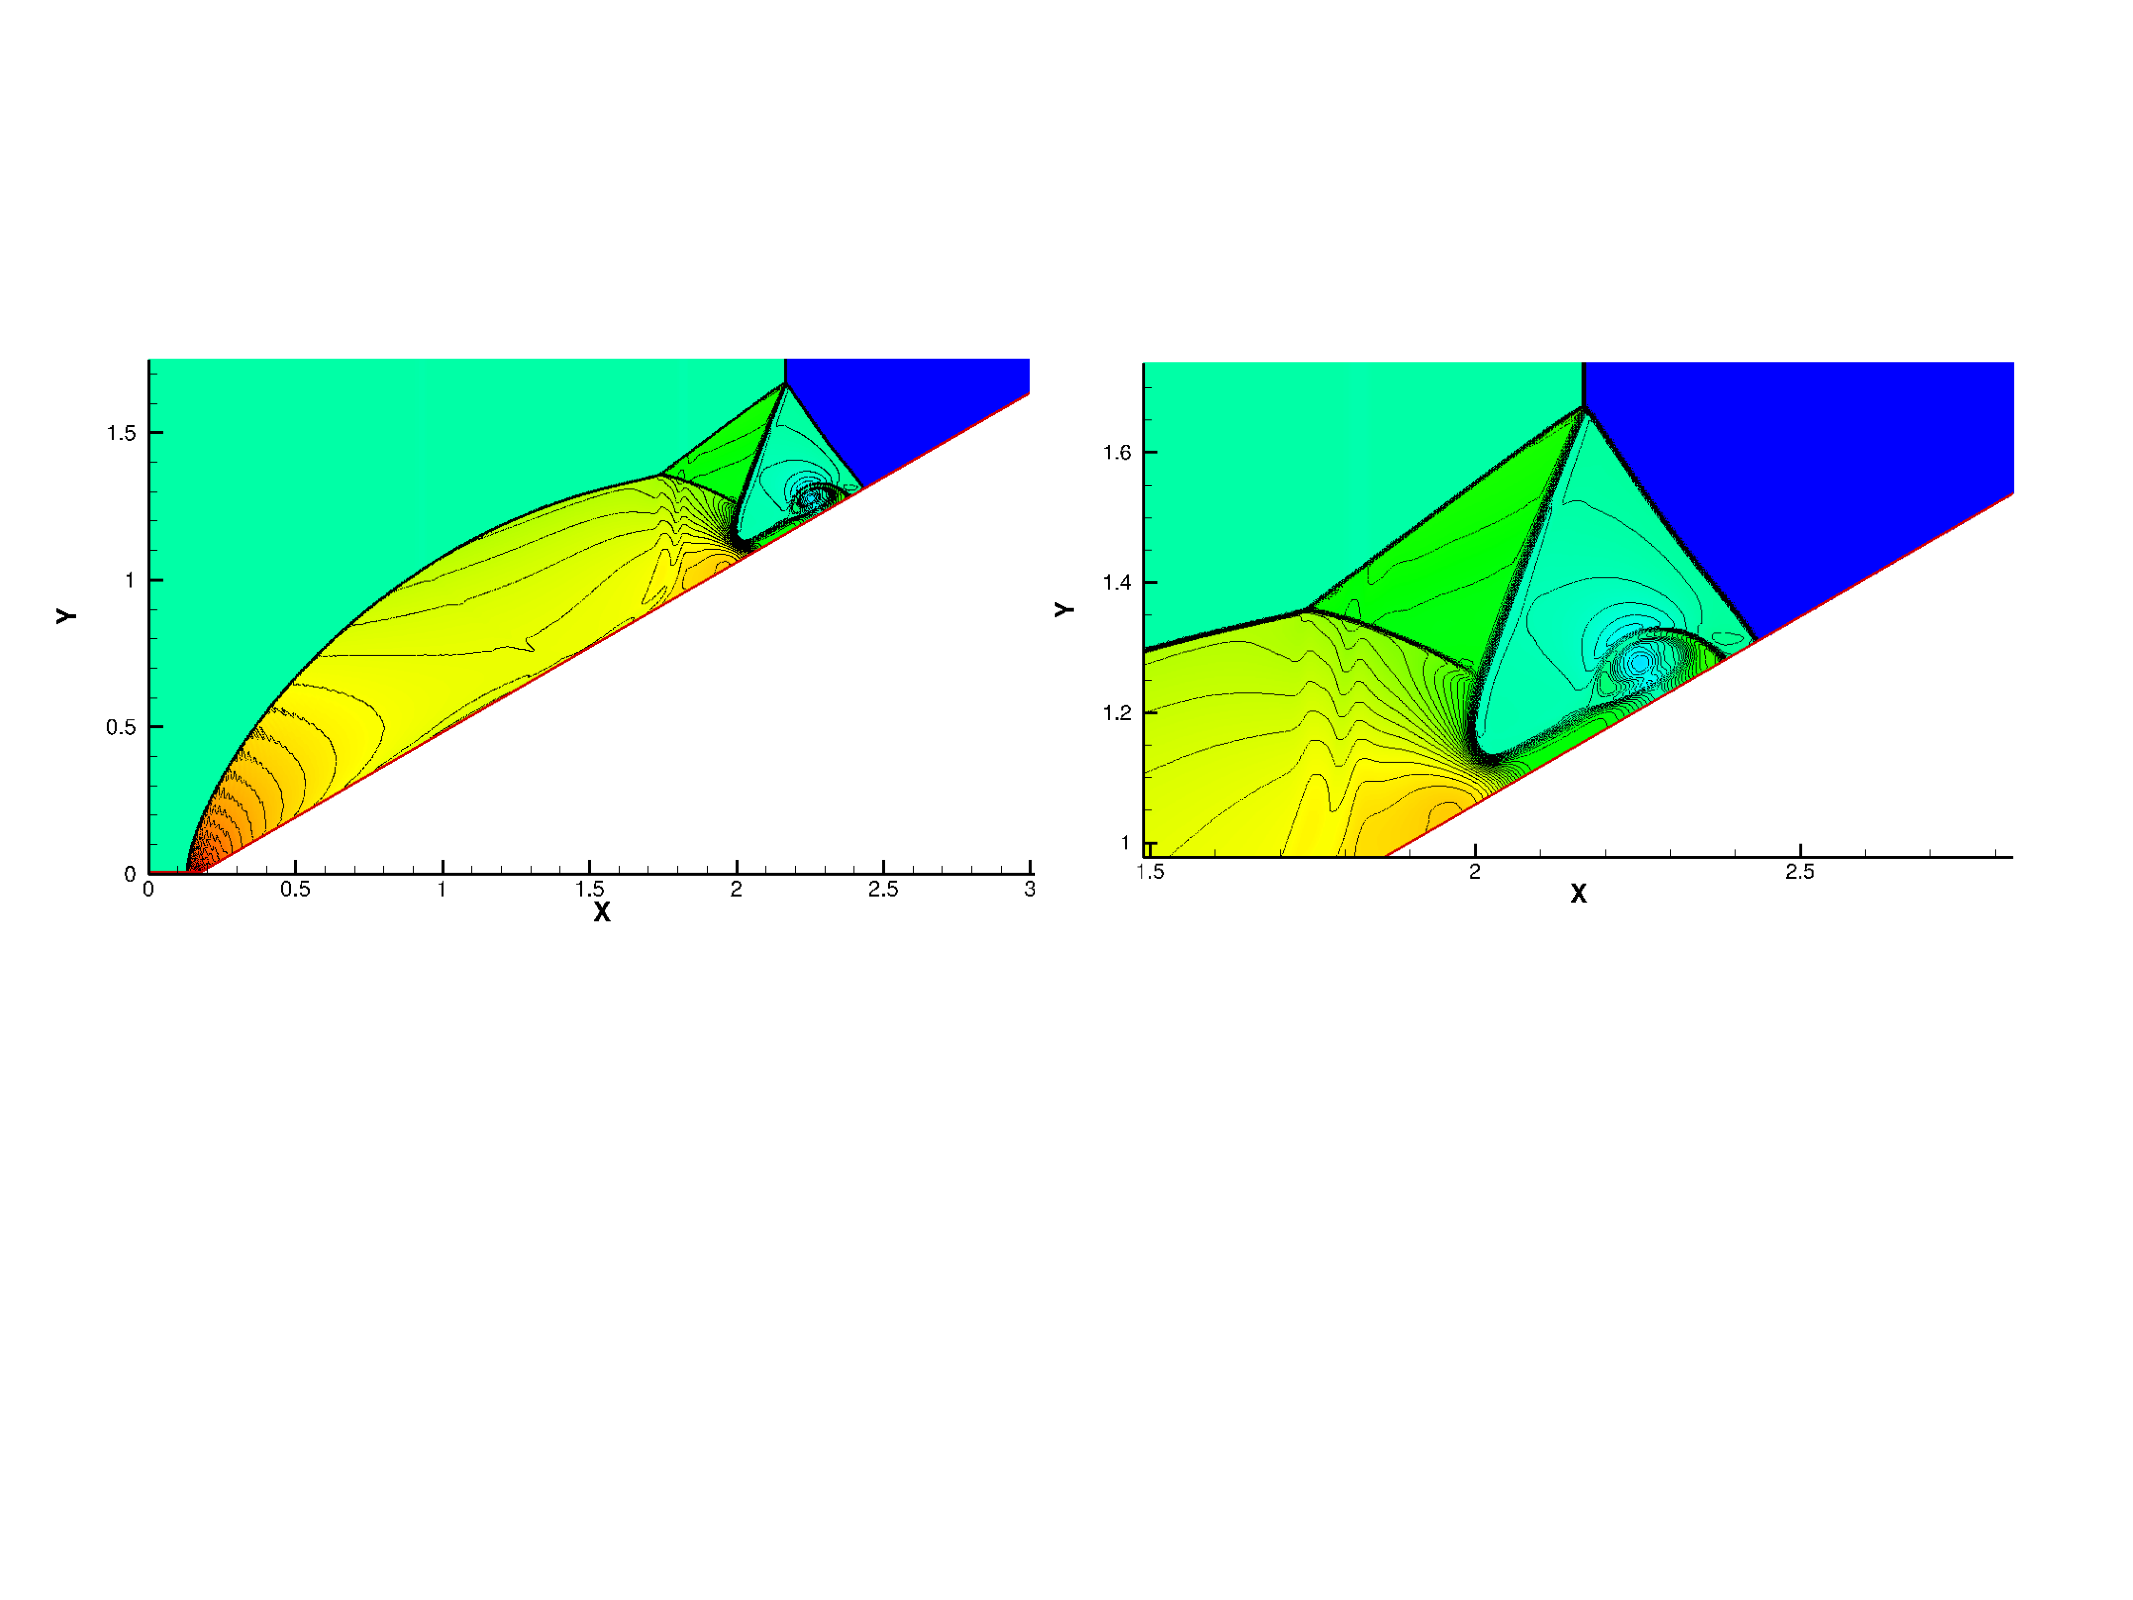
\includegraphics[width=1.1\linewidth]{figs/doubleMach480.pdf}
\caption{\sf Density plot and isolines of a Mach 10 shock impinging 
obliquely on a wedge at time $t = 0.2$ where $\Delta x = \Delta y =
1/240$ (top) and 1/480 (bottom).
The solution on the full domain is shown adjacent to a zoom of the Mach 
stem region.  Sixty isolines between 1.39 and 21.0 are drawn.}\label{fig:dm}
\end{figure}

The solution at the final time $T = 0.2$ is plotted in Figure \ref{fig:dm}, 
where the grid resolution is $\Delta x = \Delta y = 1/240$.
We obtain qualitatively comparable results to those in \cite{rkdg5} on 
the same grid resolution. We also show for comparison the results using 
$\Delta x = \Delta y = 1/480$, also done in \cite{rkdg5}. Again, the
improvement is very similar. Finally, in Figure \ref{fig:wedgeBndry} we
show the density along the boundary for the two resolutions. Despite the
irregularity of the cut cells, the solution is very smooth. The smallest
cut cell in the coarser grid has volume fraction 1.65e-6. On the finest
grid the smallest volume fraction is 2.95e-7. 

\begin{figure}[h]
\centering
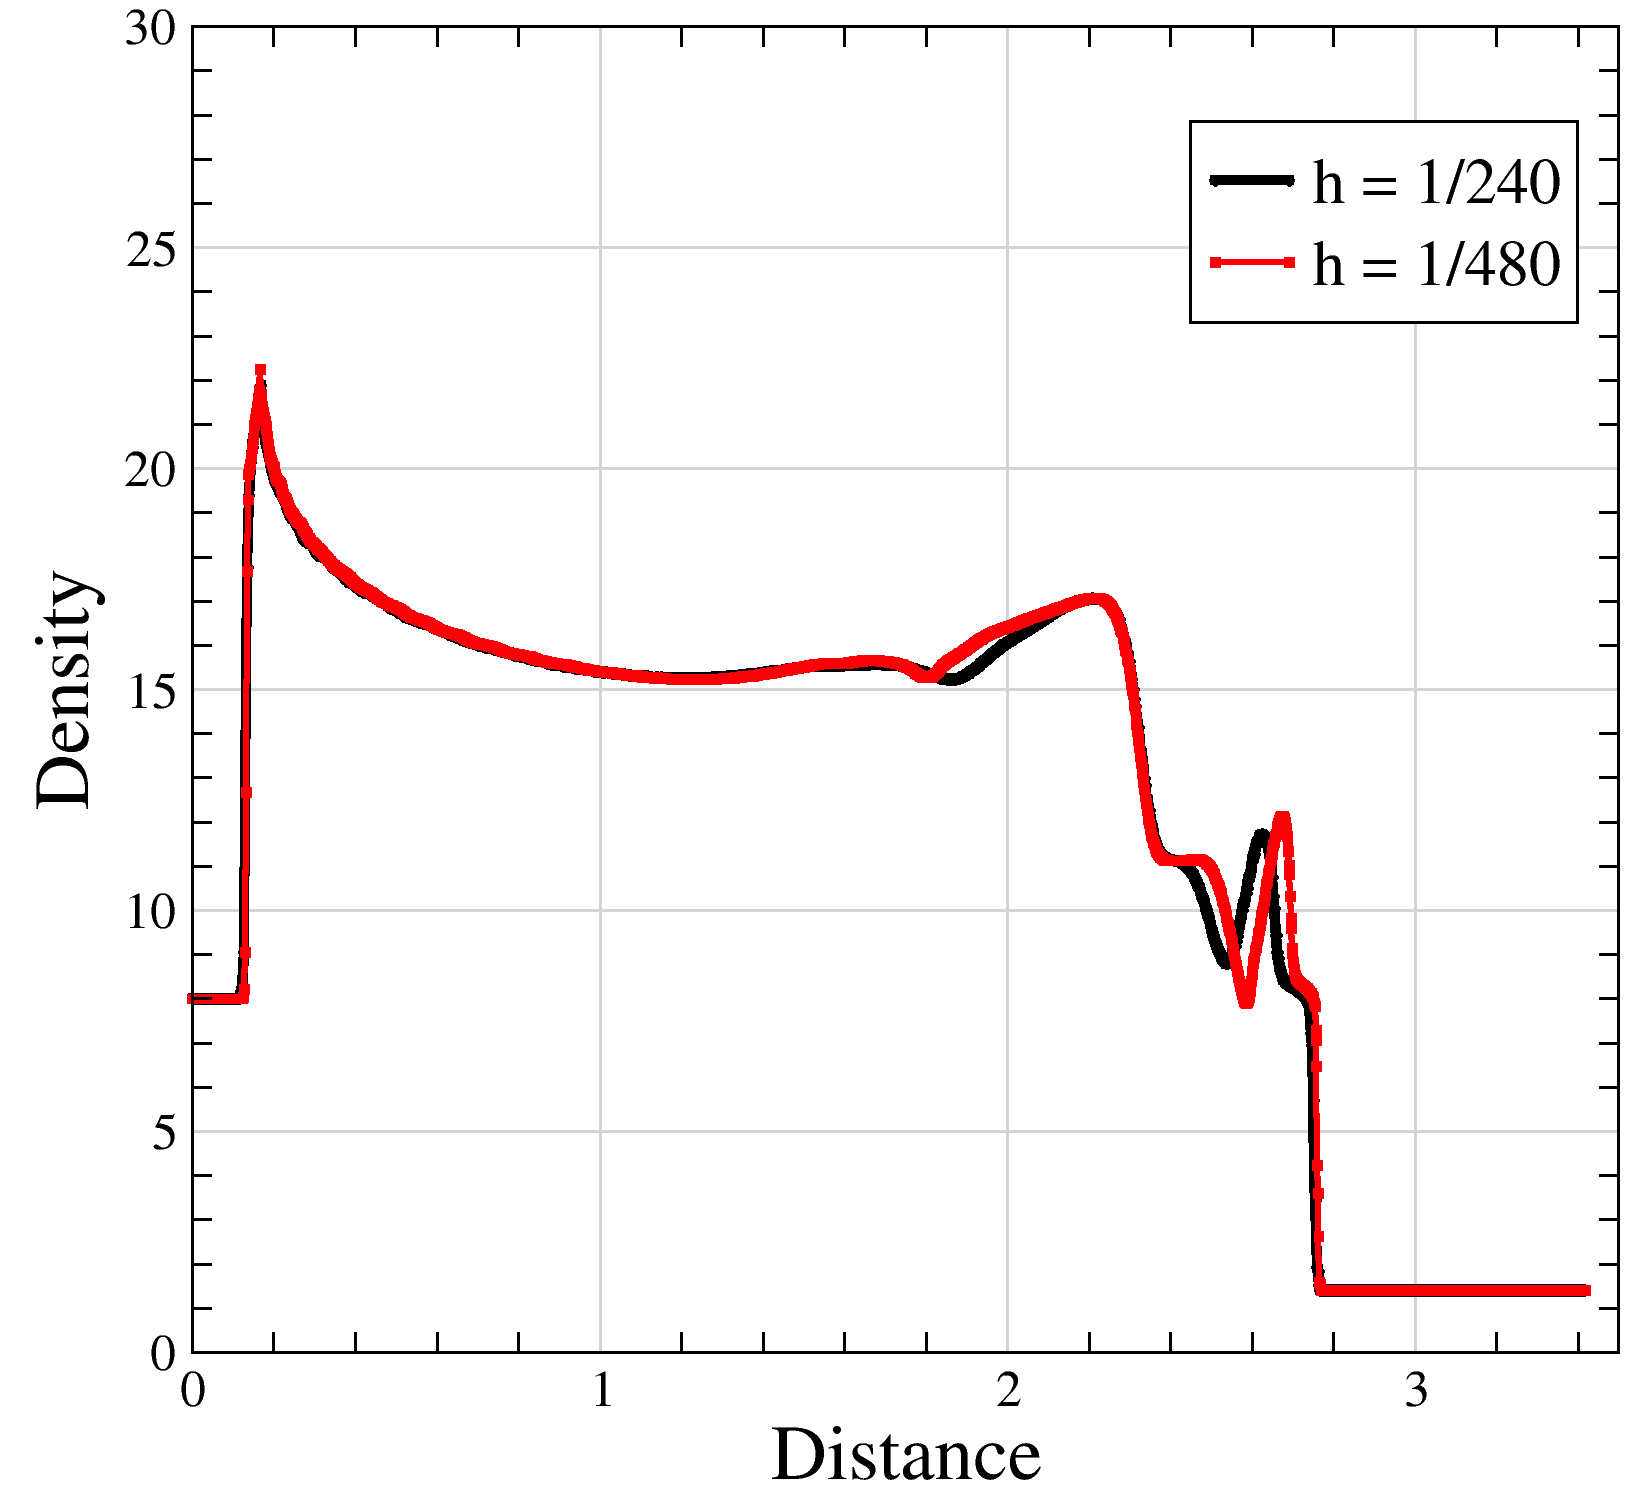
\includegraphics[width=.7\linewidth]{figs/rampWall.png}
\caption{\sf Density plotted along the wall, as a function of distance from
the lower left corner of the domain. The coarser grid has a bit of
oscillation after the ramp starts due to the curved shock. It is not due to
SRD. It is not present on the finer grid .} \label{fig:wedgeBndry}
\end{figure}


